\documentclass[preprint,12pt]{elsarticle}
% \documentclass[draft,12pt]{elsarticle}

\usepackage{hyperref}
\usepackage{graphicx}
\usepackage{subcaption}
\usepackage{amssymb}
\usepackage{amsmath}
\usepackage{multirow}
\usepackage{relsize}
\usepackage[utf8]{inputenc}
\usepackage[capitalise]{cleveref}
\usepackage{algorithm}
\usepackage[noend]{algpseudocode}
\usepackage[section]{placeins}
\usepackage{booktabs}
\usepackage{url}

% For the TODOs
\usepackage{xcolor}
\usepackage{xargs}
\usepackage[colorinlistoftodos,textsize=footnotesize]{todonotes}
\newcommand{\todoin}{\todo[inline]}
% from here: https://tex.stackexchange.com/questions/9796/how-to-add-todo-notes
\newcommandx{\unsure}[2][1=]{\todo[linecolor=red,backgroundcolor=red!25,bordercolor=red,#1]{#2}}
\newcommandx{\change}[2][1=]{\todo[linecolor=blue,backgroundcolor=blue!25,bordercolor=blue,#1]{#2}}
\newcommandx{\info}[2][1=]{\todo[linecolor=OliveGreen,backgroundcolor=OliveGreen!25,bordercolor=OliveGreen,#1]{#2}}

%Boldtype for greek symbols
\newcommand{\teng}[1]{\ensuremath{\boldsymbol{#1}}}
\newcommand{\ten}[1]{\ensuremath{\mathbf{#1}}}

\usepackage{lineno}
% \linenumbers

\journal{}

\begin{document}

\begin{frontmatter}

  \title{Study of mixing behaviour of spherical particles in fluid using stirrer}
  \author[XXX]{Dinesh Adepu\corref{cor1}}
  \ead{d.dinesh@surrey.ac.uk}
  \author[University of Surrey]{Chuan Yu Wu}
  \ead{XXX}
\address[xxx]{xxx}

\cortext[cor1]{Corresponding author}


\begin{abstract}

\end{abstract}

\begin{keyword}
%% keywords here, in the form: keyword \sep keyword
{particle dispersion}, {particle mixing}, {SPH-DEM}, {stirrer}

%% MSC codes here, in the form: \MSC code \sep code
%% or \MSC[2008] code \sep code (2000 is the default)

\end{keyword}

\end{frontmatter}

% \linenumbers


\FloatBarrier%
\section{Introduction}

Particle dispersion is a fundamental physical phenomenon encountered in
various industries where powder and fluid interactions are pivotal.  Petroleum
industry \cite{wang2023developments}, The transport of bodies in internal
systems \cite{Dai2021}, debris flow \cite{Qingyun2022}, the food processing
industry \cite{Karunasena2014}, and ice-sea modeling \cite{Mintu2018} are a
few areas to mention.  Particularly, processes involving the mixing of powder
with fluid using a stirrer are commonplace \cite{li2022study}. While
experimental investigation of such processes is often impractical due to their
highly nonlinear nature, numerical methods offer a viable alternative. These
systems are studied as part of two-way coupling models. The two-way coupling
phenomena are nonlinear, and an analytical study is not feasible. A numerical
study is preferable while handling such a phenomenon. A mesh-based or meshless
technique can be utilized to study rigid fluid coupling (RFC) numerically.
\Cref{fig:gloabl_body_frame_rb} illustrates a sample particle dispersion
problem studied in the current work.
\begin{figure}[!htpb]
  \centering
  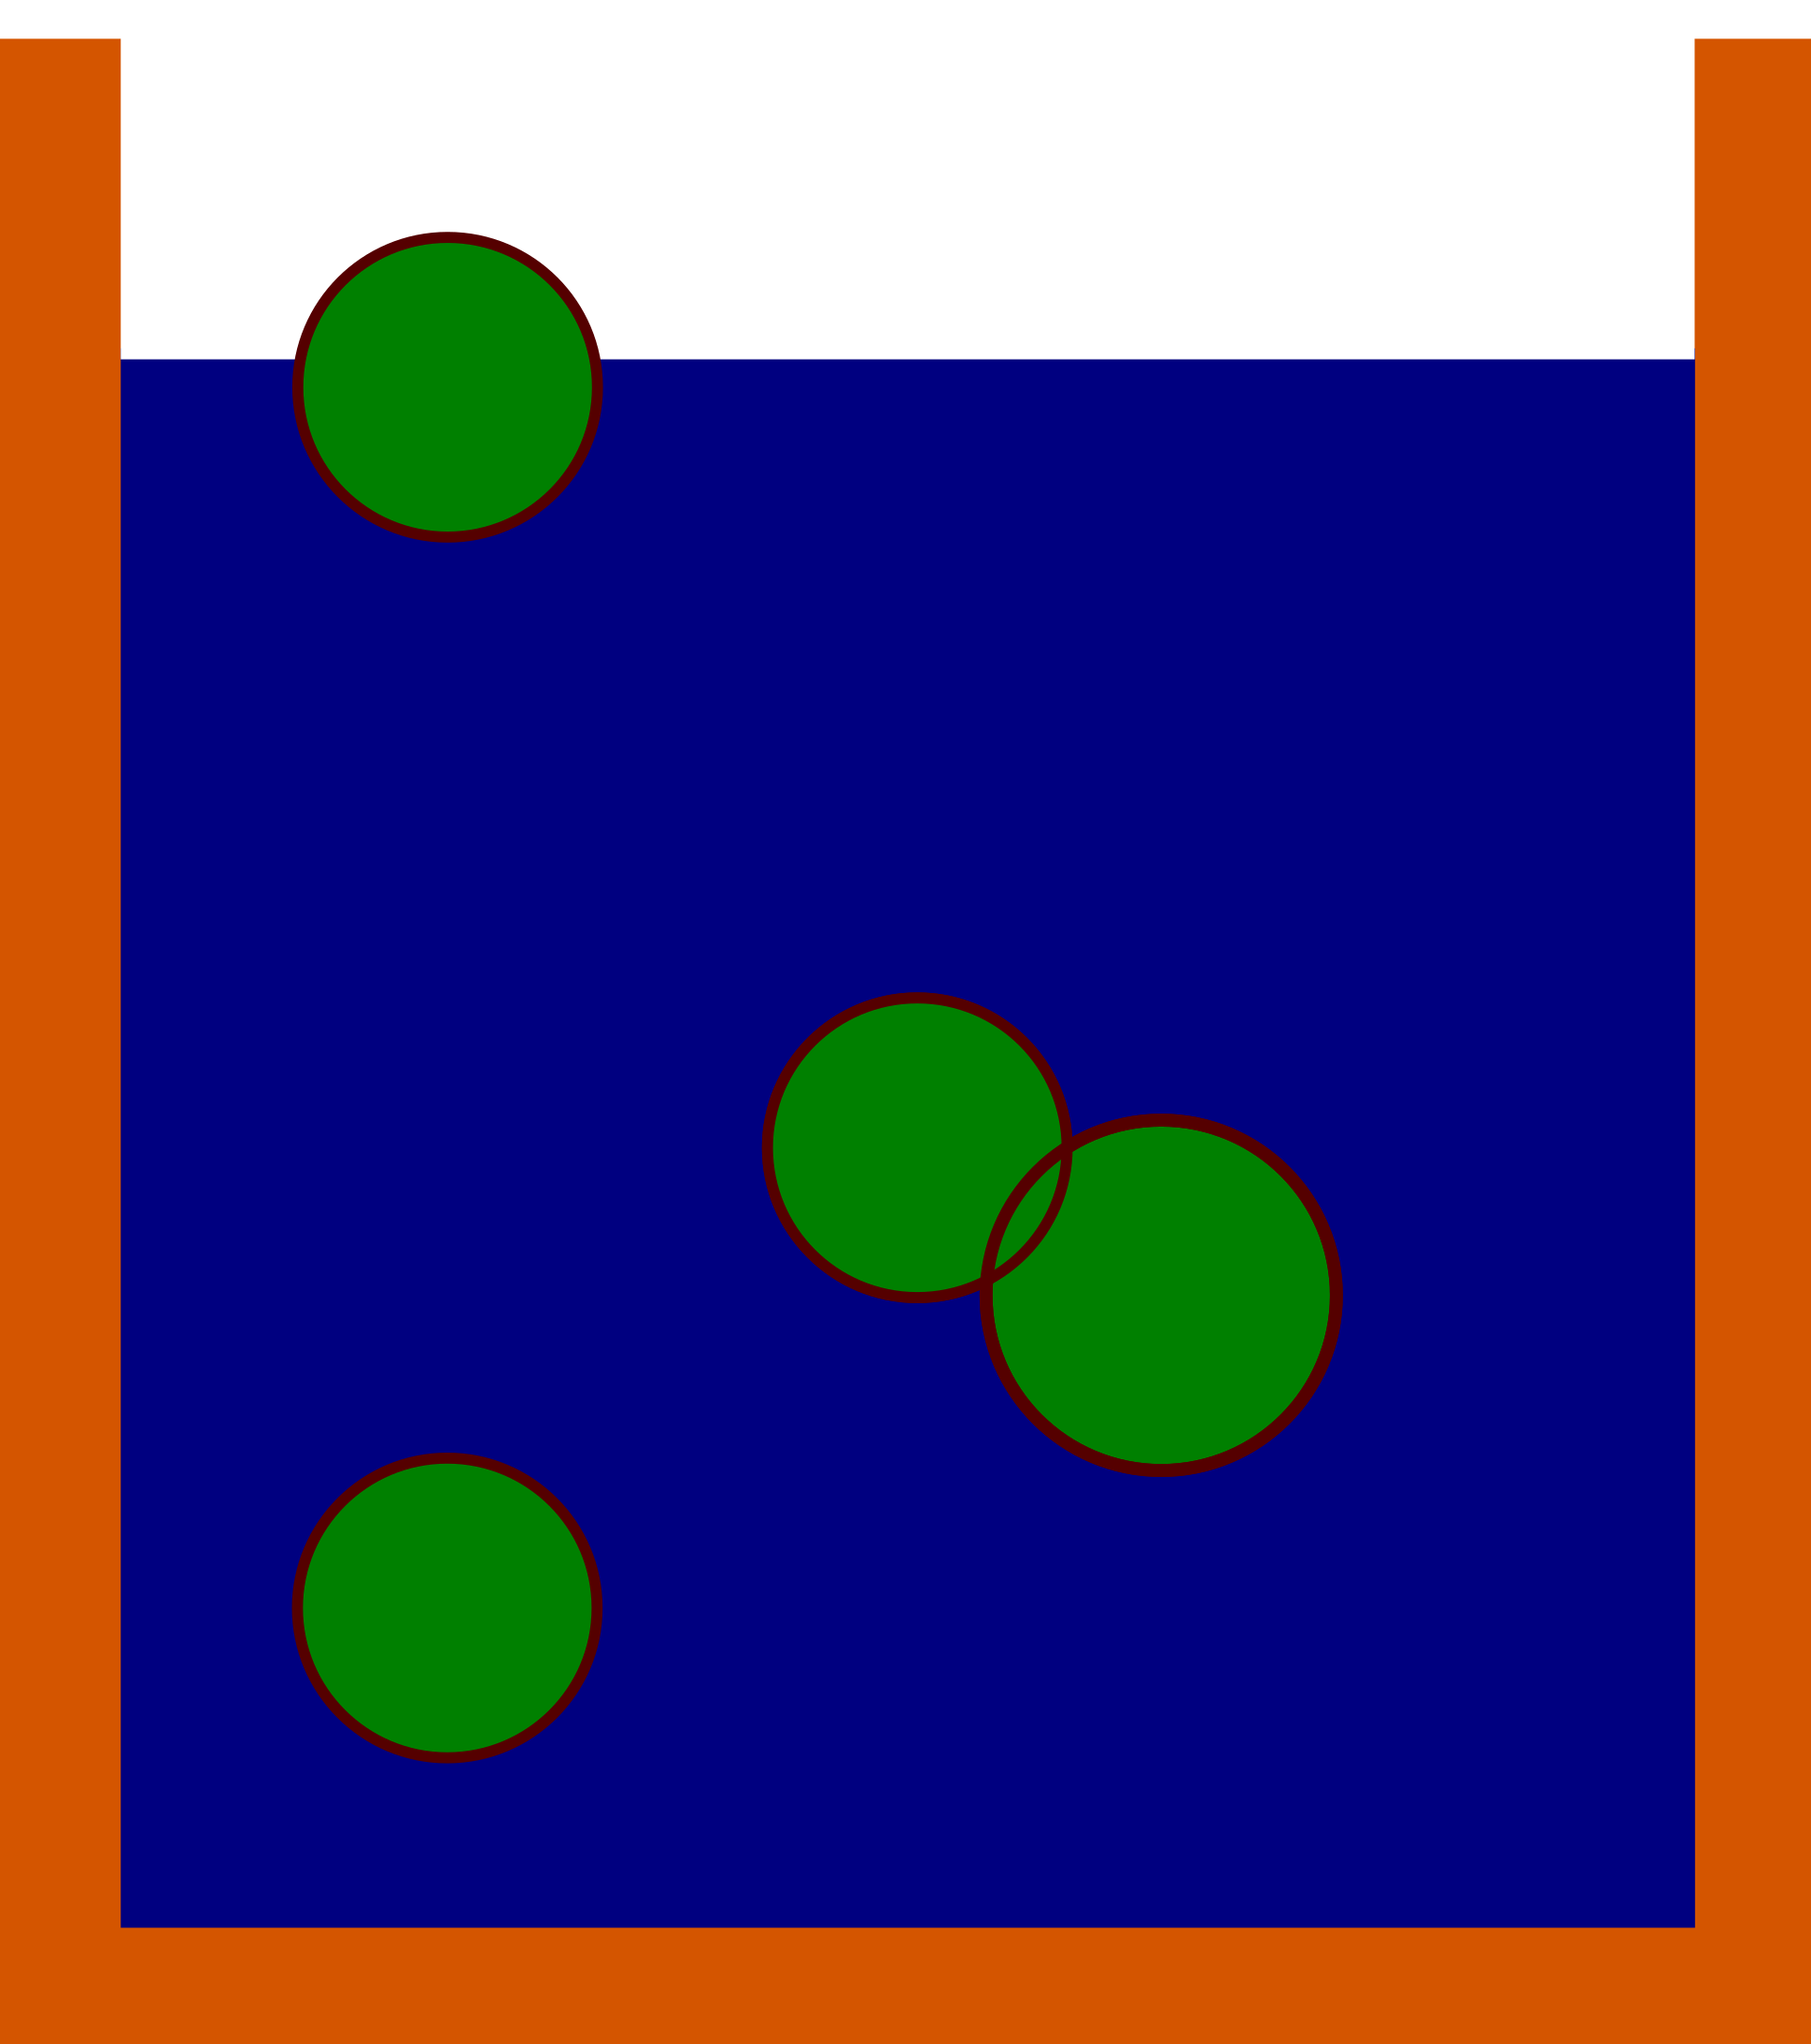
\includegraphics[width=0.4\textwidth]{images/hs_tank_fluid_with_particles}
  \caption{An illustrative figure showcasing the dispersion of particles within a free surface tank.}
  \label{intro:schematic}
\end{figure}



The combination of Discrete Element Method (DEM) for solid particle
interactions and Computational Fluid Dynamics (CFD) for fluid modeling
is a classic approach in handling particulate flow problem. In
mesh-based CFD-DEM modeling, lattice Boltzmann method (LBM)
\cite{xiong2014lbm} and finite volume method (FVM) \cite{kloss2012models} are
utilized to handle the fluid dynamics. Similarly, in meshless schemes like
Smoothed Particle Hydrodynamics (SPH) \cite{peng2021fully},
Moving Particle Semi-implicit (MPS), and Particle Finite Element
Method (PFEM) \cite{li2019modeling, franci2020pfem}, handles the fluid
dynamics.  While handling the interaction between the fluid and solid
particles, the interaction can be categorized into a resolved and unresolved
coupling. In unresolved coupling, simplified models compute forces acting on
solid particles within fluid flow, while fully resolved coupling computes
forces comprehensively. Both strategies are applicable in both meshless
\cite{cleary2015prediction, trujillo2020smooth} and mesh-based
\cite{van2008numerical, ma2022review} CFD-DEM techniques. Research such as
\cite{brosh2014accelerating} and \cite{peng2021fully} explore wide particle
size distributions with CFD-DEM and SPH-DEM respectively.  Regarding
non-Newtonian fluid modeling in mesh-based schemes, works like
\cite{li2018dam} are notable and in meshless schemes, \cite{peng2021fully} is
notable. \citet{zhu2008discrete} and \citet{ma2022review}
delve into investigations on spherical and non-spherical particles
respectively within CFD-DEM frameworks.  Meshless CFD-DEM, though fruitful,
encounters challenges in handling problems with free surfaces and becomes
computationally demanding with a large number of solid particles, especially
in fully resolved coupling. In contrast, SPH offers advantages in such
scenarios due to its inherent capability in handling free surfaces and
adeptness in modeling large mesh deformation problems, facilitating the
incorporation of novel physics.


The SPH method is a meshless numerical method originally proposed by
\citet{gingold1977smoothed} and \citet{lucy1977numerical} to model
astrophysics problems. It has been extensively applied to simulate problems
involving fluids, structural dynamics, fluid-structure interaction, granular
physics, non-Newtonian fluid flows \cite{peng2021fully} among other areas
\cite{monaghan2012smoothed}.  Various kind of particulate flows, involving,
simple spherical particles mixing using unresolved coupling
\cite{cleary2015prediction, markauskas2019coupled} and with debris
flow \cite{canelas2016sph} with fully resolved coupling approach has been
solved using SPH-DEM framework.  Handling particles of arbitrary shape in
fluid flow is addressed in various works, including those by
\citet{peng2021fully, canelas2016sph, amicarelli2015smoothed}.  Several
variants of SPH, such as WCSPH \cite{peng2021fully, cleary2015}, and ISPH
\cite{asai2021fluid}, are utilized for modeling fluid flow with particulate
flows. The coupling between fluid and rigid bodies in the fully resolved
category employs techniques such as the fixed ghost particle technique
\cite{canelas2016sph, asai2021fluid}, single layers of dummy SPH particles
\cite{peng2021fully}, and simple repulsive forces
\cite{monaghan2009sph}. Coupling between SPH fluid particles and solid
structures discretized as vertex edges is proposed by
\cite{park2023new}. Particle settling with variable sizes is studied by
\citet{zou2022study}.  Elastic behavior of spherical particles and dispersion
studies are conducted by \citet{ng2021numerical}.  Interaction between rigid
bodies of arbitrary sizes is addressed using various techniques, such as those
discussed in papers by \citet{asai2021fluid}, citet{peng2021fully},
\citet{canelas2016sph}.



In the current work we cosider the particle dispersion within a large-scale
under stirrer mixing phenomenon. We employ Smoothed Particle Hydrodynamics
(SPH) to model fluid dynamics and the Discrete Element Method (DEM) to handle
the dynamics and contact interactions among spherical particles. The
interaction between solids and fluids is managed using a fixed ghost particle
approach, ensuring a fully resolved simulation. We validate the fluid solver
independently using Poiseuille flow and the DEM solver separately using
fundamental benchmarks such as particle-particle and particle-wall
impacts. Subsequently, the fully resolved coupled SPH-DEM solver is validated
using three benchmarks: a single particle entering, two particles settling,
and a forced wedge entry into a steady hydrostatic tank. Upon confirming the
fidelity of the solver, we proceed with analyzing the mixing behavior of
various spherical particles influenced by a stirrer in a water tank. We
investigate scenarios involving particles of different densities, stirrer
velocities, and variable sizes as part of our case study. The development work
is conducted using PySPH\cite{ramachandran2021pysph}, an open-source code
available at \url{https://github.com/pypr/pysph} . To ensure reproducibility,
we utilize the automan package \cite{ramachandran2018automan} to automate all
results generated in the current manuscript, aiming for a reproducible
research approach.



The structure of this paper is as follows: In
\cref{sec:fluid-modeling}, we explain the numerical method used to model fluid
dynamics. \Cref{sec:rbd} outlines the equations governing the dynamics
of rigid bodies and the contact force model employed to resolve collisions
among them. The coupling between rigid spherical particles and the fluid is
detailed in \cref{sec:rfc}. Our results are presented in
\cref{sec:results}, where various problems from the literature are simulated to
validate the current solver, and particle dispersion is examined.



\FloatBarrier%
\section{Fluid modeling}
\label{sec:fluid-modeling}
In the current work, we follow a weakly-compressible SPH approach to model the
fluid. Smoothed particle hydrodynamics is initially developed by Lucy
\cite{lucy1977numerical} and Gingold and Monaghan \cite{gingold1977smoothed}
to model astrophysical problems. The continuum in SPH is modeled using
particles, which has physical properties such as mass, velocity, and the
particles interact based on the governing equations using a Guassian-like
kernel \cite{SPH_papers}.


\FloatBarrier%
\subsection{Fluid governing equations}
\label{sec:fluid--governing-equations}
Equations governing the fluid motion are, conservation of mass
\begin{equation}
  \label{eq:ce}
  \frac{d \rho}{d t} = - \rho \; \frac{\partial u_i}{\partial x_i},
\end{equation}
and conservation of linear momentum,
\begin{equation}
  \label{eq:me}
  \frac{d u_i}{d t} = \frac{1}{\rho} \; \frac{\partial \sigma_{ij}}{\partial x_j}
  + g_i,
\end{equation}
where $\rho$ is the density, $u_i$ is the $i$\textsuperscript{th} component of
the velocity field, $x_j$ is the $j$\textsuperscript{th} component of the
position vector, $g_i$ is the component of body force per unit mass and
$\sigma_{ij}$ is stress tensor.

The stress tensor is split into a pressure and viscous parts,
\begin{equation}
  \label{eq:fluid-stress-decomposition}
  \sigma_{ij} = - p \delta_{ij} + 2 \eta \frac{\partial u_i}{\partial x_j}
\end{equation}
where $\eta$ is the kinematic viscosity of the fluid, $p$ is the pressure,
$\delta_{ij}$ is the Kronecker delta function.


\FloatBarrier%
\subsection{Discretized fluid governing equations}
\label{sec:sph--governing-equations}
The governing equations involve function, derivative and divergence
operators. In SPH, these operators are approximated based on the positions,
mass and the kernel values of the discretized particles. Assume that the
domain is discretized into N particles with mass $m_i$ and volume
$\Delta v_i$, We have
\begin{equation}
  \label{eq:mass_repr}
  m_j = \Delta v_i \> \rho_i.
\end{equation}
Based on this discretization, the discrete function approximation is given as,
\begin{equation}
  \label{eq:discrete_form}
  A_i = \sum_{j \in \text{Neigh}(i)}\> \frac{m_j}{\rho_j} A_j\> W(\ten{x}_i - \ten{x}_j, h),
\end{equation}
where $A(\boldsymbol{x}_i) = A_i$ is the value of the field property of
particle i, similarly for $A_j$. Here, $\text{Neigh}(i)$ is the neighbours of
particle $i$.  A symmetric derivative approximation~\cite{Violeau16} is given
as,
\begin{equation}
  \nabla A(\ten{x}_i) = \rho_i \sum_{j} m_j \left(\frac{A_i}{\rho_i^2} + \frac{A_j}{\rho_j^2}\right) \nabla W_{ij}.
\end{equation}
A symmetric gradient operator ensures equal and opposite forces acting on the
particles.


An approximation of the divergence operator is used to discretize the
\cref{eq:ce}.  It is given as,
\begin{equation}
  \label{intro:eq:sph-continu-div-final}
  \nabla \cdot \ten{v}(\ten{x}_i) = \frac{1}{\rho_i} \sum_{j} m_j \left(\ten{v}_j - \ten{v}_i\right) \cdot \nabla W_{ij}.
\end{equation}


% \subsection{Discretized fluid governing equations}
The SPH discretization of the continuity
equation~\cref{eq:sph-discretization-continuity} and the momentum equation
~\cref{eq:sph-momentum-fluid} respectively are,
\begin{equation}
  \label{eq:sph-discretization-continuity}
  \frac{{d}\rho_a}{dt} = \sum_{b} \; \frac{m_b}{\rho_{b}} \;
  \rho_{a} \; {\ten{u}}_{ab} \; \cdot \nabla_{a} W_{ab},
\end{equation}

%
Similarly, the discretized momentum equation for fluids is written as,
\begin{multline}
  \label{eq:sph-momentum-fluid}
  \frac{{d}\ten{u}_{a}}{dt} = - \sum_{b} m_b
  \bigg(\frac{p_a}{\rho_a^2} + \frac{p_b}{\rho_b^2}\bigg)
  \nabla_{a} W_{ab}
 \;+\;
  \sum_{b} m_b \frac{4 \eta \nabla W_{ab}\cdot
    \ten{r}_{ab}}{(\rho_a + \rho_b) (r_{ab}^2 + 0.01 h_{ab}^2)} \ten{u}_{ab}  \;+\;
  \ten{g}_{a},
\end{multline}
where $\ten{I}$ is the identity matrix, $\eta$ is the kinematic viscosity of the
fluid and \cite{morris1997modeling} formulation is used to discretize the
viscosity term.

We add to the momentum equation an additional artificial viscosity term
$\Pi_{ab}$~\cite{monaghan-review:2005} to maintain the stability of the
numerical scheme, given as,
\begin{align}
  \label{eq:mom-av}
  \Pi_{ab} =
  \begin{cases}
\frac{-\alpha h_{ab} \bar{c}_{ab} \phi_{ab}}{\bar{\rho}_{ab}}
  & \ten{u}_{ab}\cdot \ten{r}_{ab} < 0, \\
  0 & \ten{u}_{ab}\cdot \ten{r}_{ab} \ge 0,
\end{cases}
\end{align}
where,
%
\begin{equation}
  \label{eq:av-phiij}
  \phi_{ab} = \frac{\ten{u}_{ab} \cdot \ten{r}_{ab}}{r^2_{ab} + 0.01 h^2_{ab}},
\end{equation}
%
where $\ten{r}_{ab} = \ten{r}_a - \ten{r}_b$,
$\ten{u}_{ab} = \ten{u}_a - \ten{u}_b$, $h_{ab} = (h_a + h_b)/2$,
$\bar{\rho}_{ab} = (\rho_a + \rho_b)/2$, $\bar{c}_{ab} = (c_a + c_b) / 2$, and
$\alpha$ is the artificial viscosity parameter.  The pressure $p_a$ is evaluated
using an equation of state:
\begin{equation}
\label{eqn:sph-eos}
  p_a = K \bigg(\frac{\rho_a}{\rho_{0}} - 1 \bigg).
\end{equation}
Where, $K=\rho_0 \, c_0^2$ is bulk modulus of the body, with
$c_0=10 \times V_{\text{max}}$ is speed of sound, while $\rho_0$ as the
initial density of the particles.


\FloatBarrier%
\subsection{Boundary Conditions}
\label{sec:boundary_conditions}

The ghost particle approach of \cite{Adami2012} is used to model the
boundaries. We use three layers of ghost particles to model the solid wall.
The properties of the solid wall are interpolated from the fluid particles.

When the viscous force is computed, the no slip boundary condition is used,
where the velocity on the boundary set as,
\begin{equation}
  \label{eq:no-slip-bc-u}
  \ten{u}_{\text{Ga}} = 2 \ten{u}_{\text{p}} - \ten{\hat{u}}_{\text{a}}.
\end{equation}
The projected velocity $\ten{\hat{u}}_{\text{a}}$ on the ghost particles is
computed using,
\begin{equation}
  \label{eq:v-ghost}
  \ten{\hat{u}}_a = \frac{\sum_b\ten{u}_b W_{ab}}{\sum_b W_{ab}},
\end{equation}
where $\ten{u}_b$, is the momentum velocity
of the fluid and $W_{ab}$ is the kernel value between the fluid
particle and the ghost particle.


The pressure of the boundary particle is extrapolated from its surrounding
fluid particles by the following equation,
\begin{equation}
  \label{eq:pressure-bc}
  p_w = \frac{\Sigma_f p_f W_{wf} + (\ten{g} - \ten{a}_{\ten{w}}) \cdot \Sigma_f
    \rho_f \ten{r}_{wf} W_{wf}}{\Sigma_f W_{wf}},
\end{equation}
where $\ten{a}_w$ is the acceleration of the wall. The subscript $f$ denotes
the fluid particles and $w$ denotes the wall particles.



\FloatBarrier%
\section{Rigid body dynamics}
\label{sec:rbd}
% The rigid body is discretized into particles with equal spacing each particle
% with mass $m_i$ and density $\rho_i$. Rigid body has a total 6 degrees of
% freedom (DOF), divided into $3$ translational and $3$ rotational.

% An approach using quaternions is given in \cite{dietemann2020smoothed}
% An another paper using quaternions \cite{guan2024numerical}


The equations governing the dynamics of a rigid body are, balance of linear and
angular momentum given by,
\begin{equation}
  \label{eq:rfc:balance_linear_mom}
  \frac{d \; (M \ten{v}_{cm})}{d t} = \sum_i \ten{F}_i,
\end{equation}
\begin{equation}
  \label{eq:rfc:balance_angular_mom}
  \frac{d \ten{L}}{d t} = \teng{\tau}_{cm},
\end{equation}
where $M$, $\ten{v}_{cm}$ are the mass and velocity of the center of mass of the rigid body.
$\ten{F}_i, \teng{\tau}_{cm}, \ten{L} $ are force acting at point $i$, torque and
angular momentum about the center of mass of the rigid body. In the current
case, force acting on the particle $i$, $\ten{F}_i$, is due to the interaction
with the other bodies and with the fluid particles, and any other body forces.
The torque $\teng{\tau}_{cm}$ and angular momentum $\ten{L}$ are computed as,
\begin{equation}
  \label{eq:rfc:torque}
 \teng{\tau}_{cm} = \sum_i \ten{F}_i \times (\ten{x}_{cm} - \ten{x}_{i}),
\end{equation}
\begin{equation}
  \label{eq:rfc:moi}
  \teng{L} =
  \sum_i \; \ten{r}_i \times \; (\teng{\omega} \times \ten{r}_i)
  = \sum_i \; m_i \; [(\ten{r}_i \cdot \ten{r}_i) \ten{I} - \ten{r}_i \otimes \ten{r}_i].
\end{equation}
Here $\ten{x}_{cm}$ and $\omega$ are the position of the center of mass and
angular velocity of the rigid body. $m_i$, $\ten{x}_{i}$, $\ten{r}_i$ are the
mass, position of particle, and position of particle $i$ with respect to vector
center of mass.

\begin{figure}[!htpb]
  \centering
  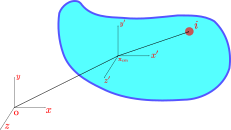
\includegraphics[width=0.7\textwidth]{images/rigid_body/rigid_body}
  \caption{Body frame and local frame description of rigid body}
  \label{fig:gloabl_body_frame_rb}
\end{figure}
We use two coordinate frames to capture the dynamics of the rigid body, a
global frame and a body frame as shown in
\cref{fig:gloabl_body_frame_rb}. The body fixed frame, which moves with
rigid body is always located at the center of mass ($\ten{x}_{cm}$). The
state of the rigid body at a given time ($t$) can be described using position
($\ten{x}_{cm}$) and velocity ($\ten{v}_{cm}$) of the center of mass, a
rotation matrix($\ten{R}$) to represent the orientation of the rigid body with
respect to the global frame, and angular velocity($\teng{\omega}$). The center
of mass is computed as
\begin{equation}
  \label{eq:rfc:center_of_mass}
  \ten{x}_{cm} = \frac{\sum_i m_i \; \ten{x}_{i} }{\sum_i m_i }.
\end{equation}
The position of the discretized particle ($i$) in
\cref{fig:gloabl_body_frame_rb} belonging to the rigid body at time $t$ can be
computed as,
\begin{equation}
  \label{eq:rfc:rb_particle_pos_update}
  \ten{x}_i = \ten{x}_{cm} + \ten{r}_{i},
\end{equation}
with
\begin{equation}
  \label{eq:rfc:rb_particle_pos_update}
  \ten{r}_i = \ten{R} \overline{\ten{r}}_{i}.
\end{equation}
Here $\overline{\ten{r}}_{i}$ is the position of the particle $i$ about the body
frame axis and remains constant through out the simulation. The rotation matrix
$\ten{R}$ is used to bring the body frame position vector to the global frame
$\ten{O}$. Similarly the velocity vector is computed as,
\begin{equation}
  \label{eq:rfc:rb_particle_vel_update}
  \ten{v}_i = \ten{v}_{cm} + \teng{\omega} \times \ten{r}_{i}.
\end{equation}

We evolve the state of the rigid body through the integration of the
\cref{eq:rfc:balance_linear_mom,eq:rfc:balance_angular_mom}. The linear velocity of the
center of mass ($\ten{v}_{cm}$) and angular momentum ($\ten{L}$) at the next
timestep are computed as,
\begin{equation}
  \label{eq:rfc:lin_vel_cm_update}
  \ten{v}_{cm}^{n+1} = \ten{v}_{cm}^{n} + \frac{\ten{F}_{cm}}{M} \; \Delta t,
\end{equation}
\begin{equation}
  \label{eq:rfc:ang_mom_update}
  \ten{L}^{n+1} = \ten{L}^{n} + \teng{\tau}_{cm} \; \Delta t.
\end{equation}
Here, $\ten{F}_{cm} = \sum_i \ten{F}_i$.

The position of the center of mass and the rotation matrix ($\ten{R}$) are updated
by,
\begin{equation}
  \label{eq:rfc:lin_pos_cm_update}
  \ten{x}_{cm}^{n+1} = \ten{x}_{cm}^{n} + \ten{v}_{cm}^{n} \; \Delta t,\\
  \ten{R}^{n+1} = \ten{R}^{n} + \tilde{\teng{\omega}}^{n} \, \ten{R}^{n} \; \Delta t,
\end{equation}
where $\tilde{\teng{\omega}}^{n}$ is matrix formulation of angular velocity
$\omega$. The angular velocity at the new time step is computed with
\begin{equation}
  \label{eq:rfc:ang_velocity_update}
  \teng{\omega}^{n+1} = (\textit{\teng{I}}^{-1})^{n+1} \; \ten{L}^{n+1}.
\end{equation}
Here, moment of inertia at the new time step is computed as,
\begin{equation}
  \label{eq:rfc:moi_update}
  (\textit{\teng{I}}^{-1})^{n+1} = \ten{R}^{n+1} \textit{\teng{\overline{I}}}^{-1} (\ten{R}^{n+1})^T.
\end{equation}
where moment of inertia ($\textit{\teng{\overline{I}}}^{-1}$) in body frame is
used to compute in global frame at every time instant for faster computations.
The moment of inertia ($\textit{\teng{\overline{I}}}$) is computed as,
\begin{equation*}
\textit{\teng{\overline{I}}} =
\begin{bmatrix}
\sum_i m_i (y_i^2 + z_i^2) & -\sum_i m_i x_iy_i & -\sum_i m_i x_iz_i\\
-\sum_i m_i x_iy_i & \sum_i m_i (x_i^2 + z_i^2) &  -\sum_i m_i y_iz_i\\
-\sum_i m_i  x_iz_i & -\sum_i m_i y_iz_i & \sum_i m_i (x_i^2 + y_i^2)
\end{bmatrix}.
\end{equation*}

The position and velocity of the particles of the rigid body are updated by
\begin{eqnarray}
  \label{eq:rfc:rb_particle_pos_update}
  \ten{r}_i = \ten{R} \cdot \overline{\ten{r}}_{i},\\
  \ten{x}_i = \ten{x}_{cm} + \ten{r}_{i},\\
  \ten{v}_i = \ten{v}_{cm} + \teng{\omega} \times \ten{r}_{i}.
\end{eqnarray}

The force acting on particle $i$ is composed of interaction with the other rigid
bodies, and the fluid, given as
\begin{eqnarray}
  \label{eq:rfc:rb_particle_pos_update}
  \ten{F}_i = \ten{F}_{\text{Fl}}^i + \ten{F}_{\text{cont}}^i
\end{eqnarray}
We follow \cref{sec:dem} to compute force
$\ten{F}_{\text{cont}}^a$ acting on particle $i$ due to the interaction with
the rigid bodies. The force $\ten{F}_{\text{rfc}}^i$ acting due to the
interaction with the fluid particles follows \cref{sec:rfc}.



\FloatBarrier%
\subsection{Contact resolution}
\label{sec:dem}

\begin{figure}[!htpb]
  \centering
  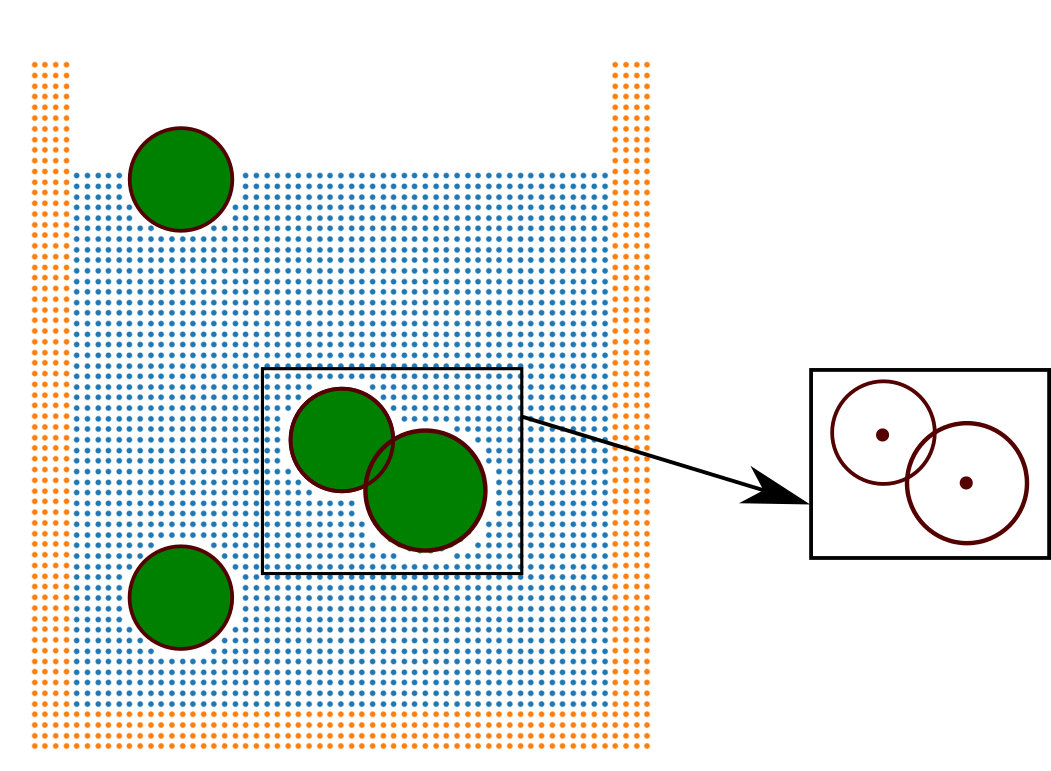
\includegraphics[width=0.7\textwidth]{images/spherical_particles_dem_representation}
  \caption{Demonstration of contact handling between two rigid spherical
    particles immersed in a fluid tank.}
  \label{fig:spherical-particles-in-tank-dem}
\end{figure}

We resolve the contact among the spherical particles using discrete element
method. In the current work we have utilized a non-linear contact force
model. In DEM, the force acting on a particle $a$ due to the interaction with
the particle $b$ is resolved into a normal and tangential component. The
normal force component is utilised to make sure that the particle do not
penetrate into each other, while the tangential component is used to model the
friction between the interacting particles.  The normal force
($\teng{F}_a^{n}$) on particle $a$ due to the interaction with the particles
$b$ is given by a non-linear, Hetzian model \citet{brilliantov1996model},
\begin{equation}
  \label{eq:contact-algorithm-normal}
  \ten{F}_a^n = k_r \delta_{n} \ten{n}.
\end{equation}
Here, the overlap $\delta_{n}$ is computed using
\begin{equation}
  \label{eq:cf-overlap}
  \delta_{n} = R_{a} + R_{b} - r_{ab},
\end{equation}
$k_r$ is the normal spring stiffness coefficient, which is computed using the
material properties of the bodies in contact \cite{golshan2023lethe}.


\subsection{Tangential force computation}
\label{sec:tangential-force-computation}
To handle the frictional contact, we associate a tangential spring attached to
particle $a$ and particle $b$ to compute the tangential force, which initially has
a magnitude of zero ($|\Delta \textit{\textbf{l}}_a|=0$). The tangential spring
is activated when the particle comes into contact with particle $b$. The
tangential force is history-dependent. The contact friction force is
proportional to the tangential spring displacement, which is integrated over
the contact time as
\begin{equation}
  \label{eq:tangential-force}
  \ten{F}_{a}^{t^{n+1}} =
  -k_f \Delta \textit{\textbf{l}}_a^{\,n + 1} =
  -k_f \big[\big(\Delta {\textit{\textbf{l}}}_a^{\,n} \
  + \ten{v}_{ab}^{n + 1} \Delta t\big) \cdot \ten{t}_a^{n + 1} \big] \
  \ten{t}_a^{n + 1},
\end{equation}
where $\Delta t$ is the time step, $\ten{v}_{ab} = \ten{v}_{a} - \ten{v}_b$ is the
relative velocity of particle $a$ with respect to the contacting particle $b$,
and $k_f$ is the tangential spring stiffness coefficient. The tangential
spring stiffness is computed similar to the normal spring
stiffness\cite{golshan2023lethe}.  The tangential unit vector is computed by,
\begin{equation}
  \label{eq:tangential-vect}
  \ten{t}_a = \frac{\ten{v}_{ab} - (\ten{v}_{ab} \cdot \ten{n}) \ten{n}}{|\ten{v}_{ab} - (\ten{v}_{ab} \cdot \ten{n}) \ten{n}|}.
\end{equation}

The tangential force is coupled to the normal force through the Coulomb's law,
\begin{equation}
  \label{eq:Coulomb-law}
  \ten{F}_{a}^{t} = \min(\mu |\ten{F}_{a}^{n}|, |\ten{F}_{a}^{t}|) \
  \frac{\ten{F}_{a}^{t}}{|\ten{F}_{a}^{t}|}.
\end{equation}
This allows us to impose the sliding friction condition between the
interacting solids. Finally, the total force acting on the particle $a$ due to
the interaction with particle $b$ is:
\begin{equation}
  \label{eq:contact-force}
  \ten{F}_{a}^{\text{cont}} = \ten{F}_{a}^{n} + \ten{F}_{a}^{t}
\end{equation}

An equal and opposite force of the same magnitude is applied to
particle $b$, given as
\begin{equation}
  \label{eq:contact-force}
  \ten{F}_{b}^{\text{cont}} = - \ten{F}_{a}^{\text{cont}}.
\end{equation}



\FloatBarrier%
\section{Rigid fluid coupling}
\label{sec:rfc}

% Coupling equation with single particles he2017coupled
% Coupling with dummy particles \cite{guan2024numerical}
% A different coupling equation meng2022hydroelastic

\begin{figure}[!htpb]
  \centering
  \begin{subfigure}{0.22\textwidth}
    \centering
    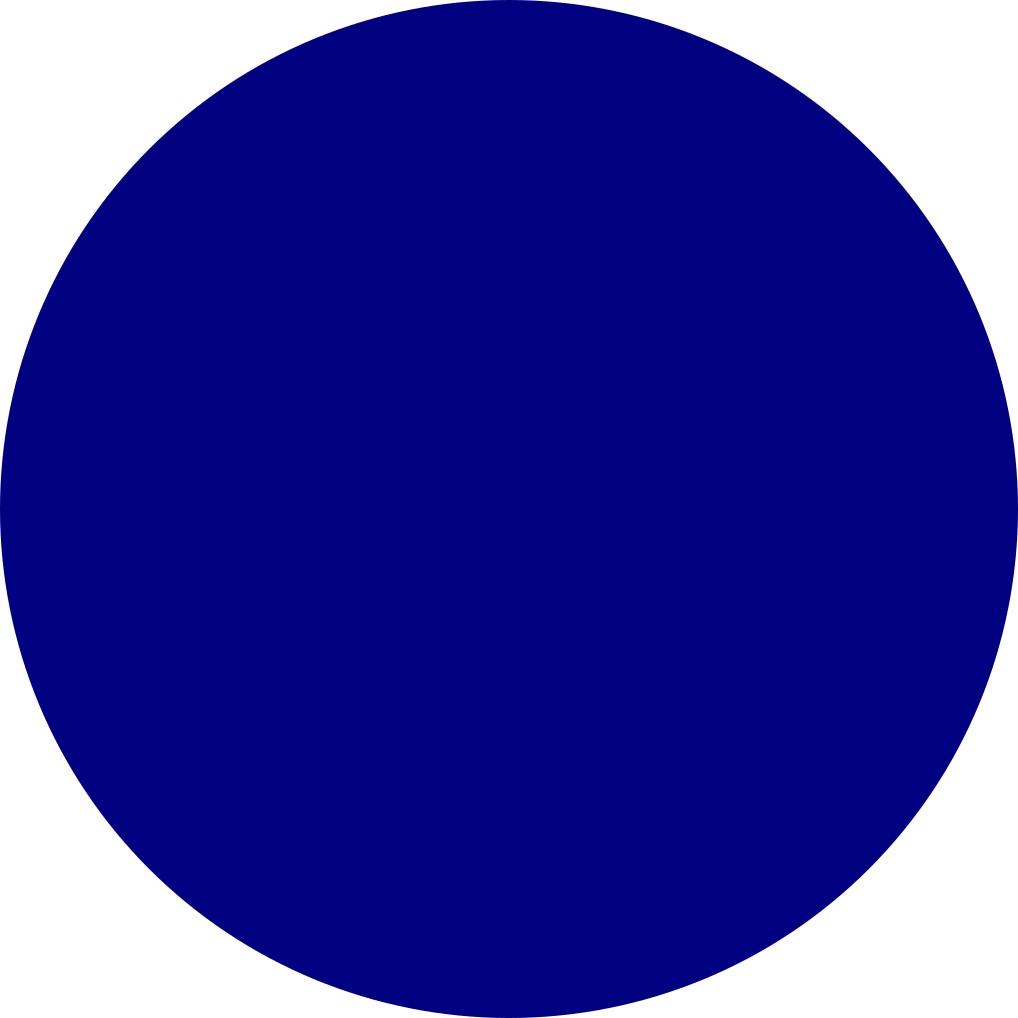
\includegraphics[width=1.0\textwidth]{images/rfc_explantion_schematic/real_spherical_particles}
    \subcaption{A rigid spherical particle}%\label{fig:rings:ipst-nu-0.47-0}
  \end{subfigure}\hspace{15mm}%
  \begin{subfigure}{0.24\textwidth}
    \centering
    
\includegraphics[width=1.0\textwidth]{images/rfc_explantion_schematic/sph_sampled_spherical_particles}
    \subcaption{A rigid spherical particle sampled with dummy SPH particles}%\label{fig:rings:ipst-nu-0.47-1}
  \end{subfigure}
  \caption{}
\label{fig:real_particle_sph_sampling}
\end{figure}
To calculate the force exerted on the spherical particle by the surrounding
fluid, we employ a method involving the sampling of the spherical particle
using dummy Smoothed Particle Hydrodynamics (SPH) particles, depicted in
\cref{fig:real_particle_sph_sampling}. These SPH particles are evenly
distributed and remain stationary, moving in tandem with the velocity of the
rigid particle at any given location. To establish the pressure of these SPH
particles, we utilize the fixed ghost particle boundary technique outlined in
\cref{sec:boundary_conditions}.



With spherical particles being discretized into SPH particles and immersed in
fluid can be seen in \cref{fig:many_rb_in_fluid_sph_particles}.
\begin{figure}[!htpb]
  \centering
  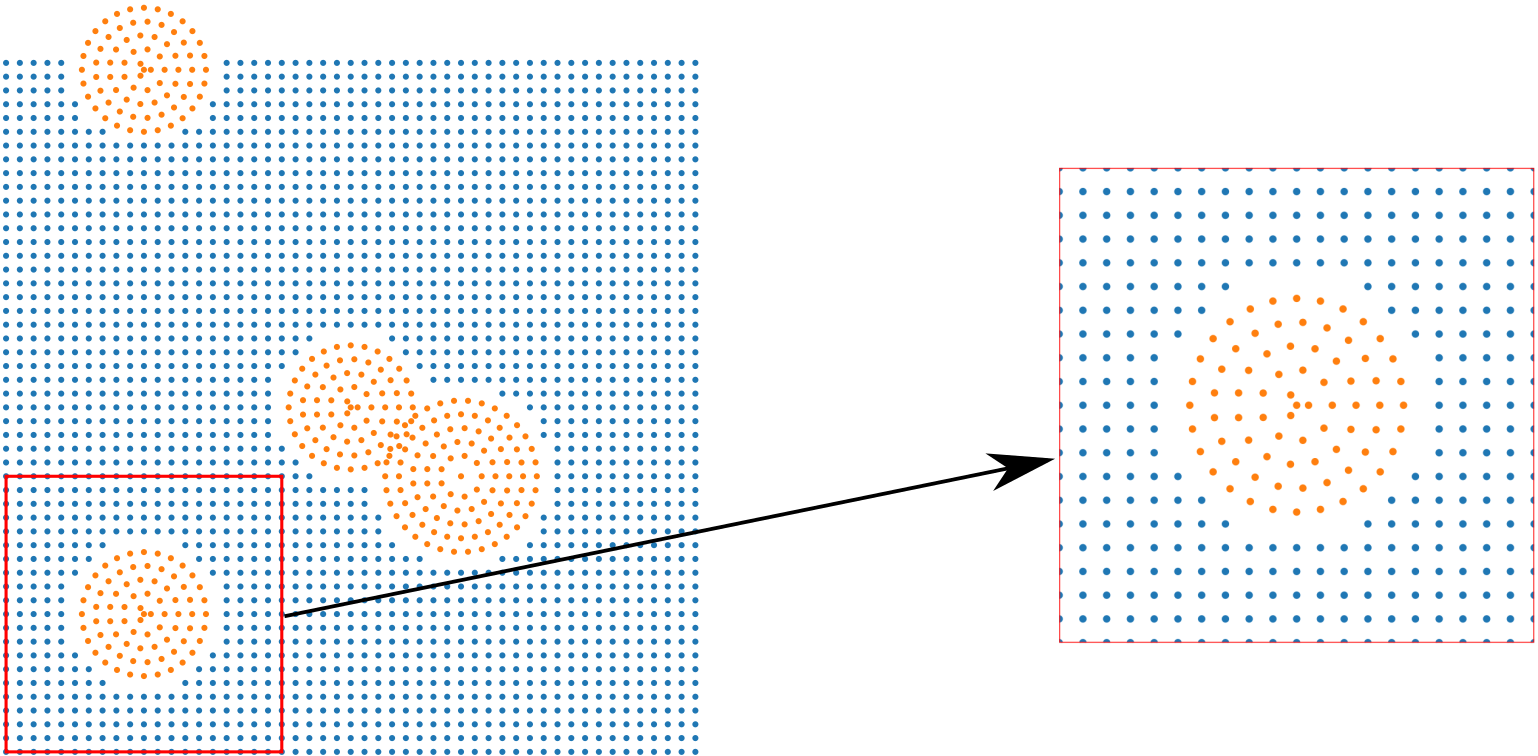
\includegraphics[width=0.7\textwidth]{images/rfc_zoomed_combined}
  \caption{A rigid spherical particle sampled with dummy SPH particles being
    immersed in a fluid tank. An SPH particle representation}
  \label{fig:many_rb_in_fluid_sph_particles}
\end{figure}
The force on the fluid particle due to the
interaction with the sampled dummy SPH particles is considered in the momentum
\cref{eq:sph-momentum-fluid} and the continuity
\cref{eq:sph-discretization-continuity}. The force acting on the sampled dummy
SPH particle due to the interaction with the fluid is given by,
\begin{equation}
  \label{eq:rfc-force}
  \ten{F}_{\text{rfc}}^a = -m_a \sum_{f} m_f \bigg(\frac{p_f}{\rho_{f}^2} +
  \frac{p_a}{\rho_{a}^2}\bigg) \nabla_{a} W(x_{af}).
\end{equation}
Here, $m_a$ signifies the hydrodynamic mass of the sampled dummy SPH particle,
and $\rho_a$ represents its hydrodynamic density. While $m_f$, $p_f$ and
$\rho_f$ are mass, pressure and density of the fluid particle.


\FloatBarrier%
\section{Time Integration}

We use the kick-drift-kick scheme for the time integration. We move the
velocities of the fluid and the solid particles to half time step,
\begin{equation}
  \label{eq:velocity-update-stage-1}
  \ten{u}_a^{n+\frac{1}{2}} = \ten{u}_a^{n} + \frac{\Delta t}{2} \bigg(\frac{d\ten{u}_{a}}{dt}\bigg)^n,
\end{equation}
Then the time derivative of density is calculated using the
\cref{eq:sph-discretization-continuity} using the velocities at half time
step. The new time step density and particle position is updated by,
\begin{equation}
  \label{eq:density-update-stage-2}
  \rho_{a}^{n+1} = \rho_{a}^{n} + \Delta t \; \bigg(\frac{d\rho_{a}}{dt}\bigg)^{n+\frac{1}{2}},
\end{equation}
\begin{equation}
  \label{eq:position-update-stage-2}
  \ten{r}_{a}^{n+1} = \ten{r}_{a}^{n} + \Delta t \; \ten{u}_{a}^{n+1}.
\end{equation}
%
Finally, at new time-step particle position, the momentum velocity is updated
\begin{equation}
  \label{eq:velocity-update-stage-3}
  \ten{u}_a^{n+1} = \ten{u}_a^{n+\frac{1}{2}} + \frac{\Delta t}{2} \bigg(\frac{d\ten{u}_{a}}{dt}\bigg)^{n+1}.
\end{equation}


The modeling of rigid-rigid interaction requires lower time step than the
fluid. We choose the minimum of both the timesteps to move the system forward
in time. For the numerical stability of fluid, the time step depends on the
CFL condition as,
\begin{equation}
  \label{eq:rfc:time-step-cfl}
  \Delta t_{\text{fluid}} = \mathrm{min} \bigg( 0.25 \; \frac{h}{c + |U|} ,  0.25 \; \frac{h^2}{\nu},  0.25 \; \frac{h^2}{g} \bigg),
\end{equation}
where $|U|$ is the maximum velocity magnitude, $c$ is the speed of sound
typically chosen as $10 |U|$ for fluids in this work. For rigid body, the time
step is constrained as,
\begin{equation}
  \label{eq:rfc:time-step-body-force}
  \Delta t_{\text{rb}} \leq \frac{\pi}{50} \sqrt{\frac{m}{k_r}}.
\end{equation}
A minimum timestep is chosen as
\begin{equation}
  \label{eq:rfc:time-step-body-force}
  \Delta t = min(\Delta t_{\text{fluid}}, \Delta t_{\text{rb}}).
\end{equation}



\FloatBarrier%
\section{Results}
\label{sec:results}
Initially, we validate our fluid solver through the resolution of the
Poiseuille flow problem. Subsequently, we validate the Discrete Element Method
(DEM) solver by simulating a normal head-on collision between two spherical
particles and addressing a particle-wall impact scenario. We validate the
coupled Smoothed Particle Hydrodynamics (SPH)-DEM solver is confirmed through
simulations involving a spherical particle entering a steady tank and a
falling solid in a water tank and a floating solid. Lastly, we investigate the
mixing behavior of spherical particles under a stirrer, examining cases with
varying densities and diameters.


\FloatBarrier%
\subsection{Poiseuille's flow}
\label{sec:poiseuille_flow}
% https://onlinelibrary.wiley.com/doi/epdf/10.1002/nag.898

\begin{figure}[!htpb]
  \centering
  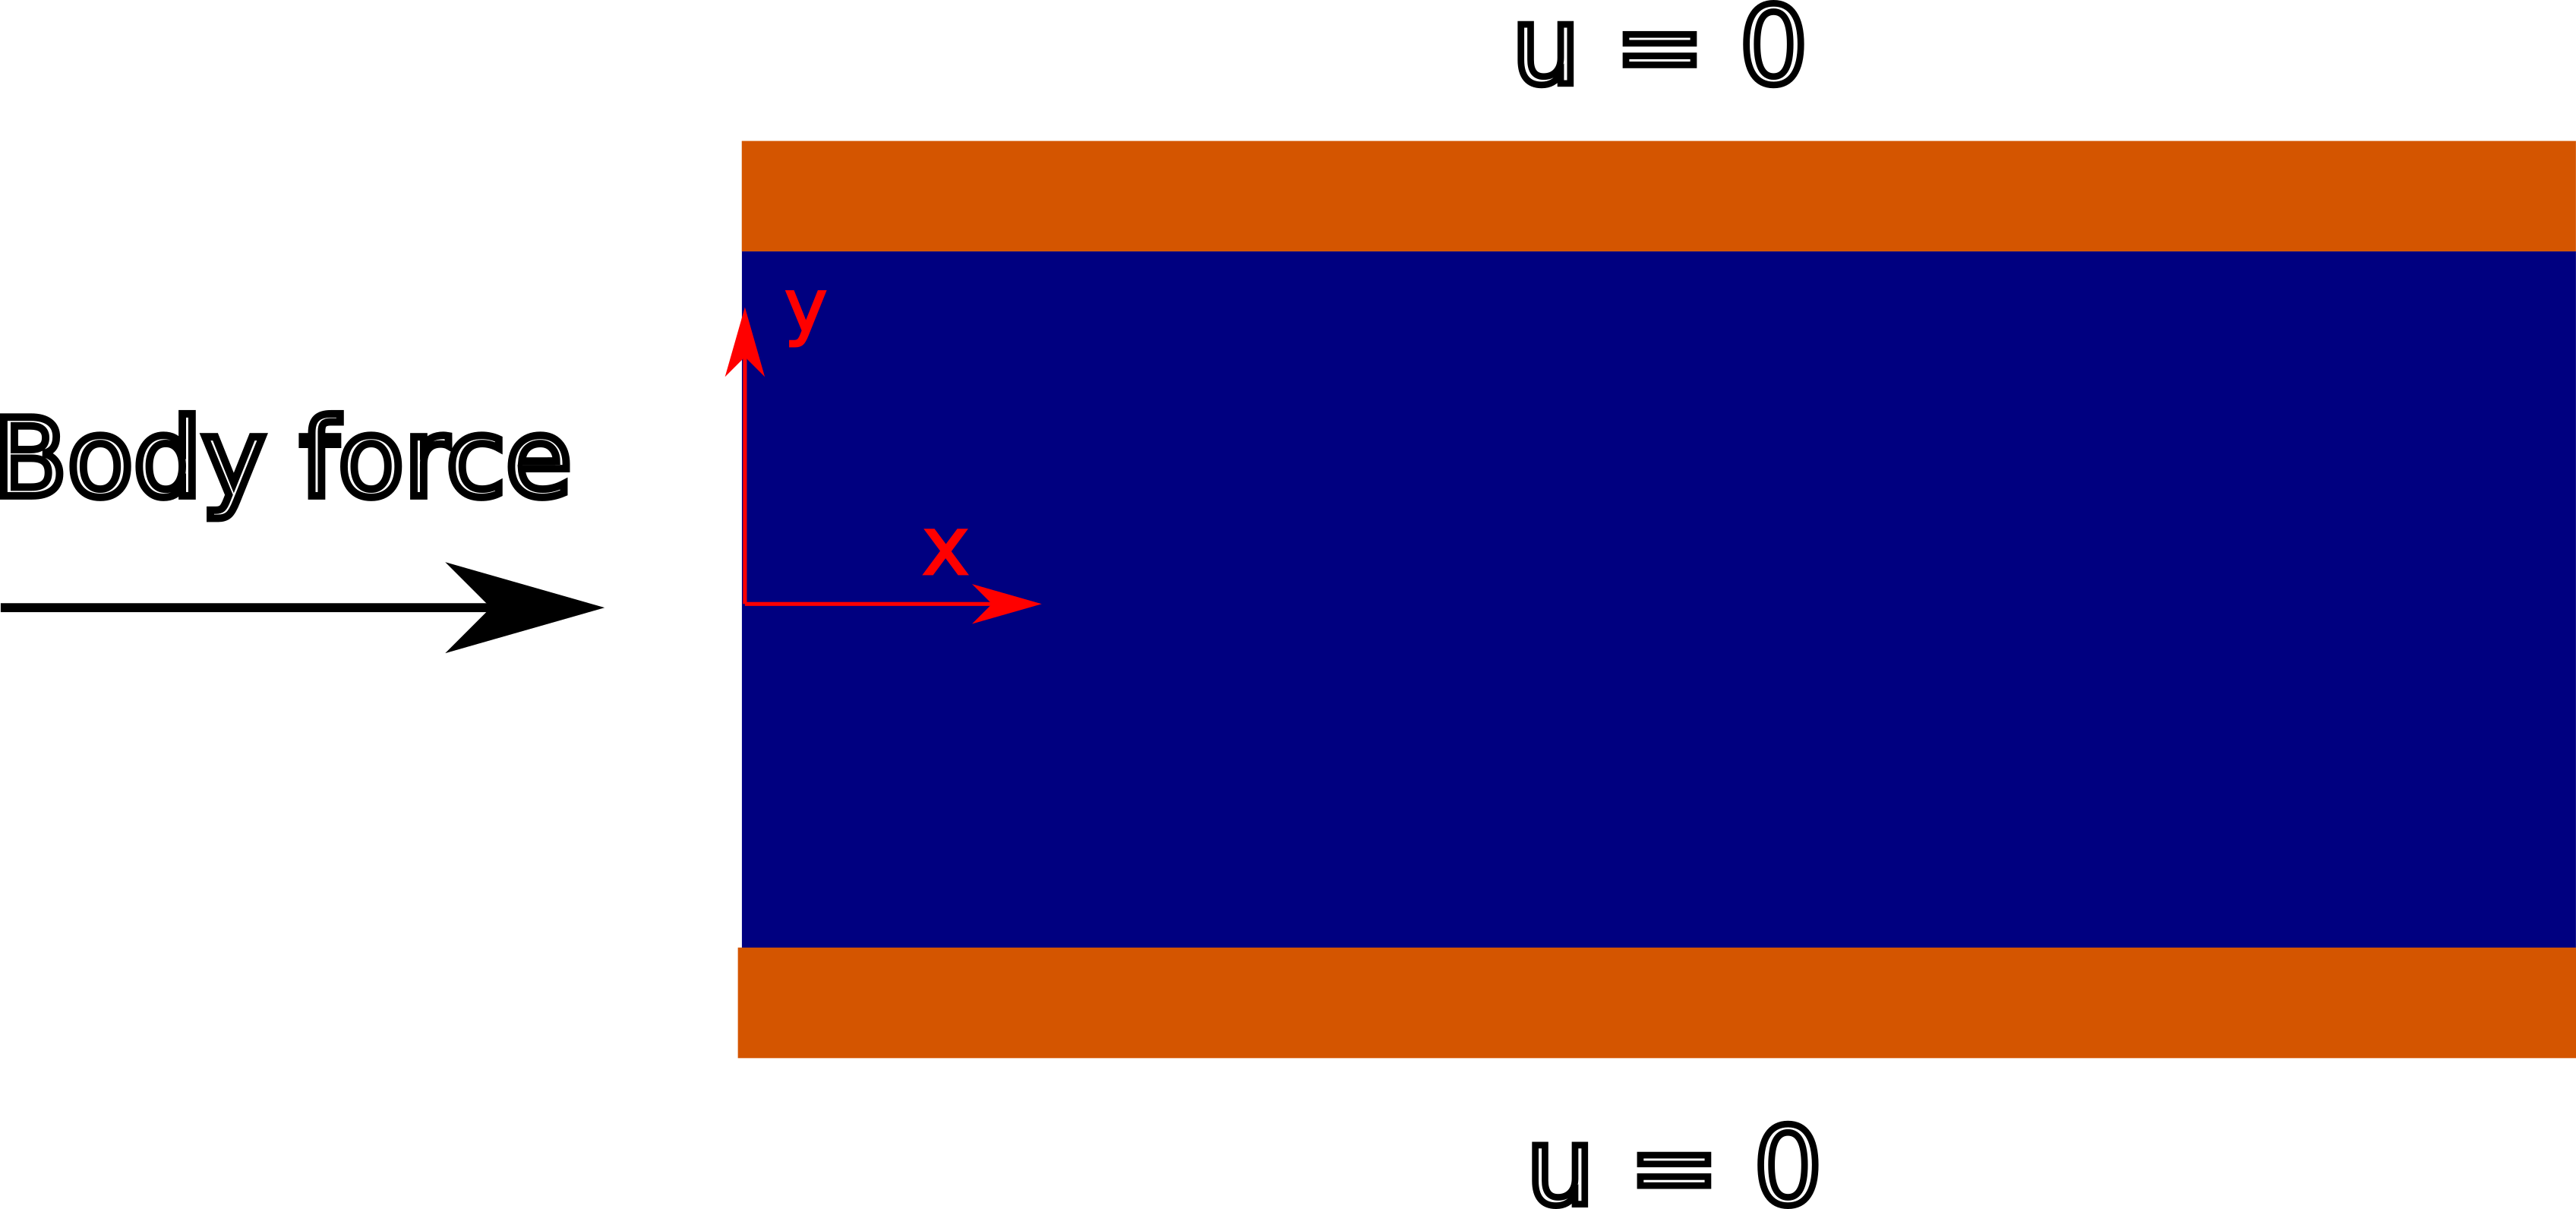
\includegraphics[width=0.7\textwidth]{images/fluid_01_benchmark_poisuelle/poiseuille_schematic}
  \caption{Poiseuille flow problem: Schematic of a fluid being driven in
    between two parlell plates due to a pressure gradient force.}
  \label{fig:poiseuille_schematic}
\end{figure}
We study unsteady flow between two infinite, parallel paltes at rest in
presence of pressure gradient to validate our fluid solver implementation.
The plates are placed $1$ m apart vertically, where the fluid is driven due to
a pressure gradient, a form of body force. The flow is towards positive x
direction. The schematic is shown in \cref{fig:poiseuille_schematic}.  In this
exact conditions, the Navier-Stokes equations admit the time dependent
solution given in \cref{eq:poiseuille_exact_soln}, as given by
\citet{morris1997modeling}
\begin{equation}
  \label{eq:poiseuille_exact_soln}
  v_x(y, t) = \frac{F}{2 \nu}y(y - L) + \sum_{n=0}^{\infty}\frac{4FL^2}{\nu \pi^3 (2n + 1)^3} \sin\bigg(\frac{\pi y}{L} (2 n + 1) \bigg) \exp\bigg(\frac{ (2 n + 1)^2 \pi^2 \nu}{L^2} t\bigg)
\end{equation}
$\nu$ is kinematic viscosity ($\frac{\mu}{\rho_0}$). This test case serves to
validate the no-slip boundary condition of our developed scheme. We use
numerical parameters such as a viscosity of $0.01$, a particle spacing of
$\frac{1}{60}$, and set the speed of sound to ten times the maximum velocity
the fluid can attain. The simulation runs for a total duration of $50$
seconds.


\Cref{fig:poiseuille_soln_graph} depicts the variation of the u-velocity in
y-direction, compared to the analytical formula given in
\cref{eq:poiseuille_exact_soln}.  By observing
\cref{fig:poiseuille_soln_graph}, we notice a close resemblance between the
SPH simulation results and the analytical solution in
\cref{eq:poiseuille_exact_soln}, thus validating our solver.
\begin{figure}[!htpb]
  \centering
  \includegraphics[width=0.4\textwidth]{figures/plane_poiseuille_flow_2D/case_1/comparison.png}
  \caption{Velocity profile of the Poiseuille flow compared against the
    analytical solution at time $t=50$ seconds.}
  \label{fig:poiseuille_soln_graph}
\end{figure}



% \FloatBarrier%
% \subsection{Rigid body validation: Dzhanibekov effect on a T-shaped rigid
% body}
% \label{sec:rb_1}
% % https://doi.org/10.1063/5.0190167



\FloatBarrier%
\subsection{DEM validation 1: Normal impact of spherical particle}
\label{sec:DEM_validation_1_normal_impact}

\begin{figure}[!htpb]
  \centering
  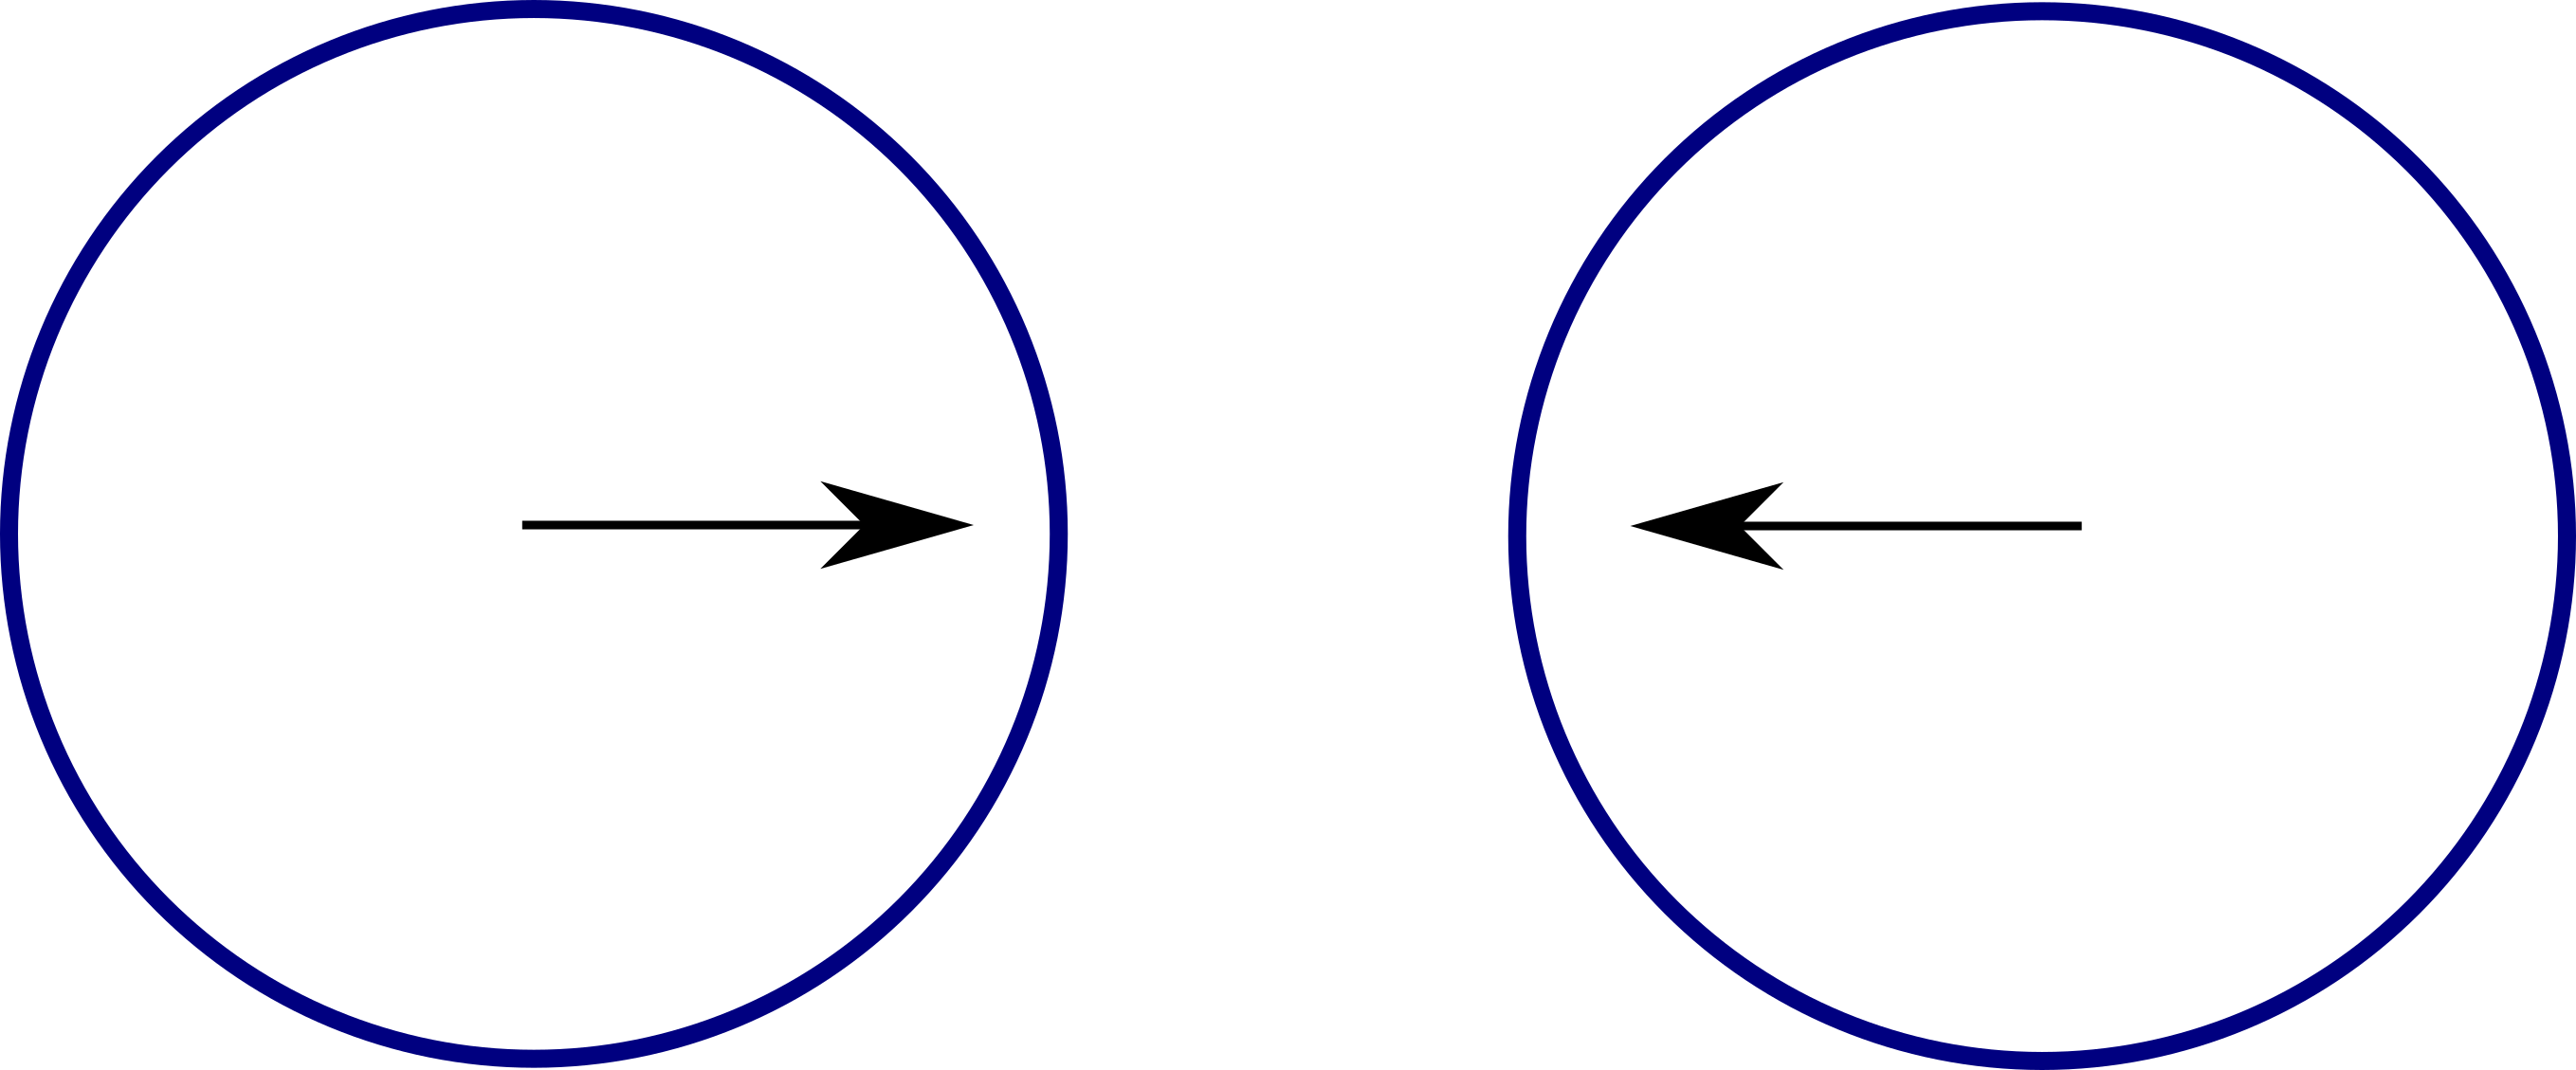
\includegraphics[width=0.6\textwidth]{images/results_dem_1_validation_particle_particle_impact/dem_01_head_on_schematic}
  \caption{Schematic of two spherical particles of equal radius in a
    head-on collision with equal magnitude of velocity but opposite direction.}
  \label{fig:result:dem_1_schematic}
\end{figure}
To validate the Discrete Element Method (DEM) solver, we analyze the direct
collision between two spherical particles.  In
\cref{fig:result:dem_1_schematic}, the initial setup depicts both particles
moving towards each other with an initial velocity of $10$
m\,s\textsuperscript{-1}.  Each disk has a radius of $0.01$ m and is composed
of glass. The glass material has a Young's modulus of $4.8 \times 10^{10}$
N\,m\textsuperscript{-2}, a Poisson ratio of $0.2$, and a density of $2800$
kg\,m\textsuperscript{-3}.  For the current scenario, we assume there is no
friction among the particles and no gravity acting on the particles.
\Cref{fig:result:dem_1_force_vs_overlap} depicts the variation of the normal
force and the amount of overlap, compared to the analytical findings presented
in \cite{chung2011benchmark}. The force curve generated by our current
implementation closely matches the analytical result, hereby confirming the
validation of our DEM solver's model for normal contact force.
\begin{figure}[!htpb]
  \centering
  \includegraphics[width=0.6\textwidth]{figures/benchmark_1_ss_colliding_elastic/fn_vs_overlap}
  \caption{Variation of the normal impact force with overlap of the impacting
    particles, compared to the analytical result.}
  \label{fig:result:dem_1_force_vs_overlap}
\end{figure}


\FloatBarrier%
\subsection{DEM validation 2: Particle wall impact}
\label{sec:DEM_validation_2_particle_wall_impact}
\begin{figure}[!htpb]
  \centering
  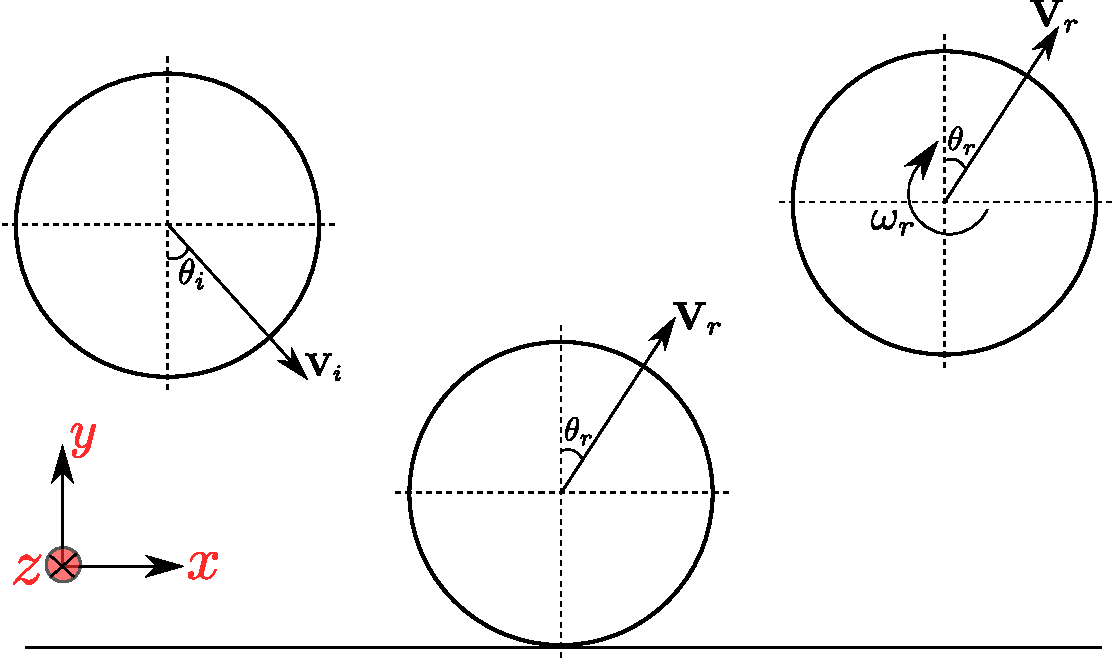
\includegraphics[width=0.6\textwidth]{images/results_dem_2_validation_particle_wall_impact/schematic}
  \caption{Schematic of a spherical particle impacting a wall
    with same magnitude of velocity but different impact angles.}
  \label{fig:result:dem_sw_contact_schematic}
\end{figure}
As part of our validation test cases, we consider the collision of a spherical
particle with wall with different incident angles and a constant velocity in
magnitude. This test case is useful in testing the tangential interaction
modeling of our DEM solver.  The current problem was experimentally
investigated by \citet{kharaz2001experimental}, and is commonly employed by
various DEM solvers to validate their codes, as seen in the work of
\cite{di2004comparison} and \cite{golshan2023lethe}.  The schematic of the
body and wall is shown in \cref{fig:result:dem_sw_contact_schematic}.
The dimensions and material properties of both the particle and the wall are
set based on the study by \cite{di2004comparison,kharaz2001experimental}. The
radius of the impacting particle is $0.0025$ m and is made of aluminium
oxide. The particle has a Young's modulus of $3.8 \times 10^{11}$
N\,m\textsuperscript{-2}, a Poisson's ratio of $0.23$, and a density of $4000$
kg\,m\textsuperscript{-3}. The wall's Young's modulus is $70\times 10^{9}$
N\,m\textsuperscript{-2}, with a Poisson ratio of $0.25$.  The impact velocity
has a magnitude of $3.9$ m\,s\textsuperscript{-1}. The coefficient of friction
between the wall and the particle is $0.092$.


In \cref{fig:result:dem_sw_contact_omega_vs_theta}, we show variation of the
rebound angular velocity with the incident impact angle, compared to
experimental data from \citet{kharaz2001experimental}.  The angular velocity
variation generated by our present implementation closely aligns with the
experimental data, thereby validating the tangential
contact model.
\begin{figure}[!htpb]
  \centering
  \includegraphics[width=0.6\textwidth]{figures/benchmark_4_sw_colliding_oblique/angle_vs_ang_vel.pdf}
  \caption{Variation of the rebound angular velocity of the impacting particle
    with the incidence angle, compared to the experimental result and Lethe
    DEM solver by \cite{golshan2023lethe}.}
  \label{fig:result:dem_sw_contact_omega_vs_theta}
\end{figure}


\FloatBarrier%
\subsection{RFC validation 1: Single particle entering into a tank}
\label{sec:rfc_validation_1_single_particle_entry}
\begin{figure}[!htpb]
  \centering
  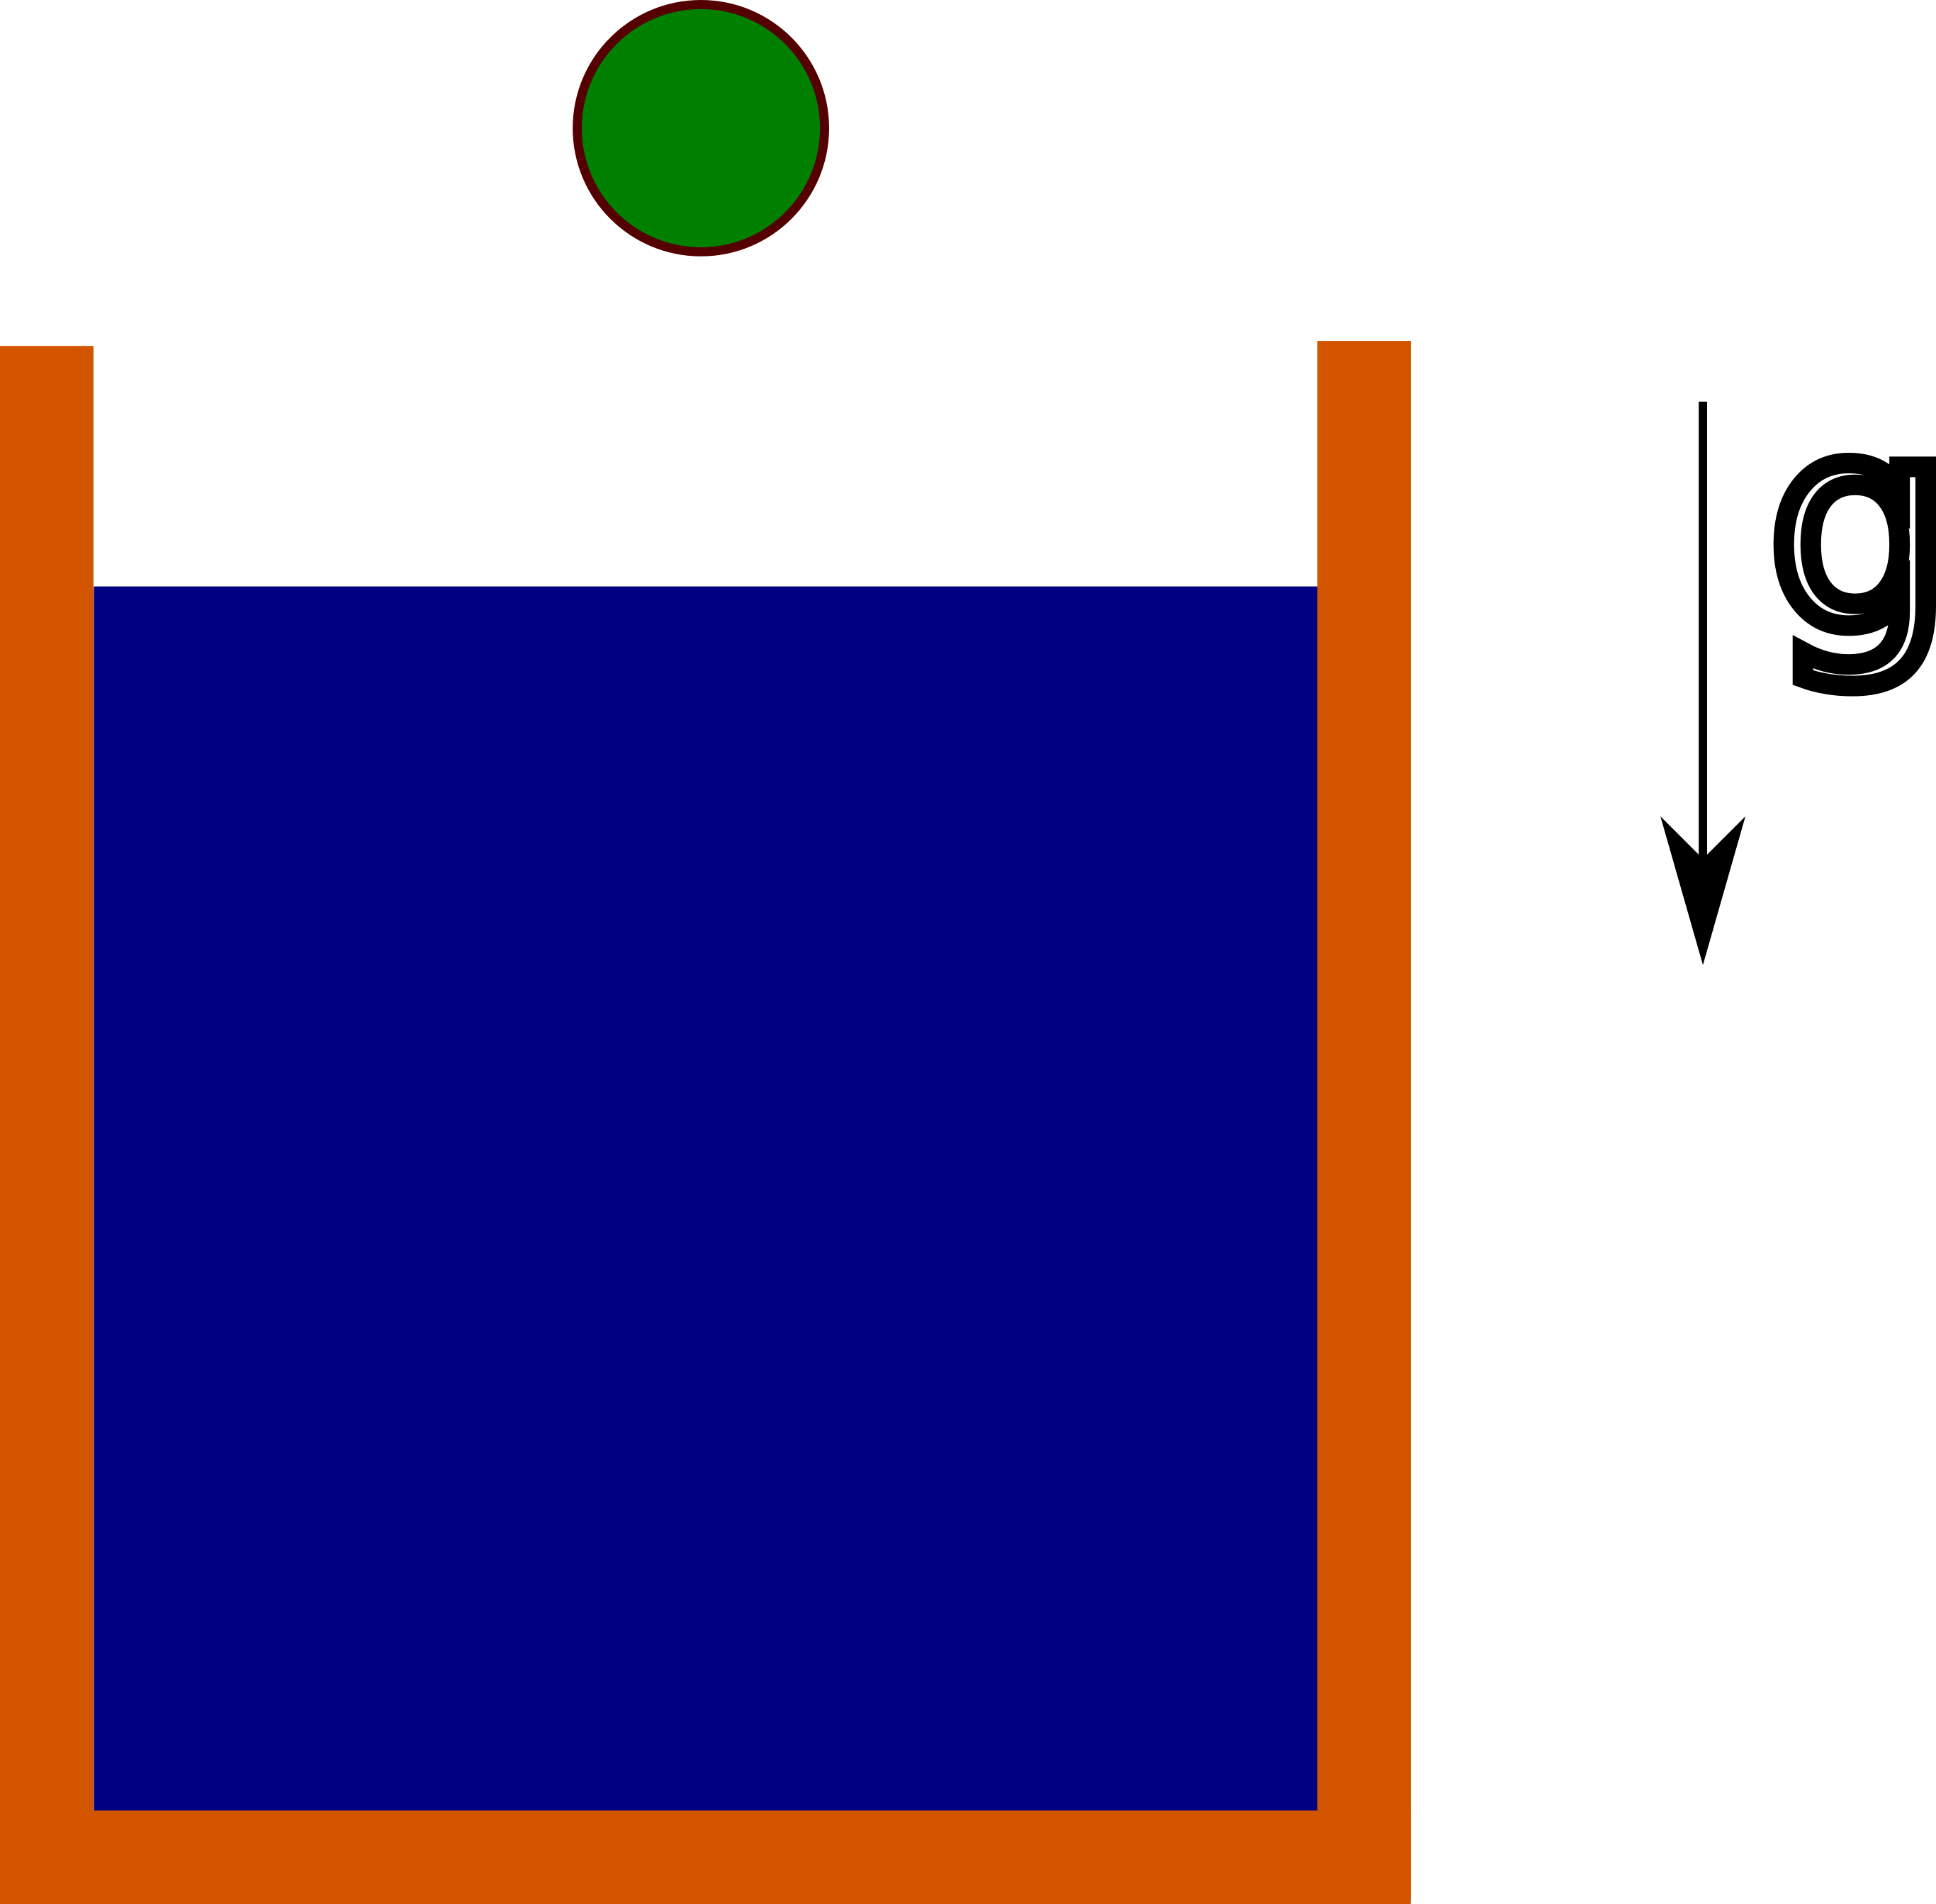
\includegraphics[width=0.4\textwidth]{images/rfc_01_skillen_2013_particle_entry_in_hs_tank/Skillen_2013_particle_entry_in_hs_tank}
  \caption{A circular cylinder entering into a calm water tank under the
    influence of the gravity.}
  \label{fig:results_rfc_01_skillen_2013}
\end{figure}

To validate the rigid-fluid coupling solver, we examine the motion of a
circular disc descending into a steady hydrostatic tank, considering two
different densities for the disc. This scenario has been investigated
experimentally by
\citet{greenhow1983nonlinear} and
numerically by various studies, including
\citet{sun2006water} using the Boundary Element Method
and \cite{sun2018accurate} employing the $\delta^+$-SPH technique.
\Cref{fig:results_rfc_01_skillen_2013}
illustrates the initial setup, with the cylinder positioned $0.5$ meters from
the free surface. The cylinder's radius is $0.11$ meters, and we investigate
cases with densities of $500$ and $1000$ kg,m\textsuperscript{-3}.
The cylinder descends due to gravity into the tank. We perform tests using
three different spacings to assess convergence: resolving the cylinder
diameter into 20, 50, and 80 particles, resulting in spacings of $5.5 \times 10^{-3}$ m,
$2.2 \times 10^{-3}$ m, and $1.375 \times 10^{-3}$ m respectively. We employ a kinematic viscosity of
$1 \times 10^{-6}$ m\textsuperscript{2}/s for water and do not utilize artificial
viscosity in this case. The simulation runs for a total time of $0.16$
seconds, utilizing a smoothing length (h) equal to the particle spacing in
each scenario. The speed of sound is set to ten times the maximum fluid
velocity attainable.


\Cref{fig:result_rfc_01_result_displacement}, depicts the evolution of the
depth of penetration of the cylinder, compared against the experimental result
by \citet{greenhow1983nonlinear}, numerical techniques of boundary element
method (BEM)(\cite{sun2006water}) and delta-plus SPH
(\cite{sun2018accurate}). From \cref{fig:result_rfc_01_result_displacement},
we find that the current numerical results matches well with the experimental result as
well as the numerical studies and also converges while increasing the
resolution.
\begin{figure}[!htpb]
  \centering
  \begin{subfigure}{0.48\textwidth}
    \centering
    \includegraphics[width=1.0\textwidth]{figures/skillen_2013_water_entry_half_buoyant/penetration_vs_t}
    \subcaption{Half buoyant cylinder}%\label{fig:rings:ipst-nu-0.47-0}
  \end{subfigure}
  \begin{subfigure}{0.48\textwidth}
    \centering
    \includegraphics[width=1.0\textwidth]{figures/skillen_2013_water_entry_neutrally_buoyant/penetration_vs_t}
    \subcaption{Neutrally buoyant cylinder}%\label{fig:rings:ipst-nu-0.47-1}
  \end{subfigure}
  \caption{Variation of the penetration depth of the cylinder with time,
    compared to BEM model \cite{sun2006water} and $\delta$+SPH model\cite{sun2018accurate}.}
\label{fig:result_rfc_01_result_displacement}
\end{figure}


\FloatBarrier%
\subsection{RFC validation 2: A 3D cube falling in water}
\label{sec:rfc_validation_2_falling_solid_in_water}

The current test case involves falling of a solid cube in a calm water
tank. The position of the cube is compared with the
experimental\cite{wu2014two} result for the validation of the current SPH-DEM
solver. This problem has been used as a standard benchmark in validating
several other numberical techniques, such as in VOF-DEM solver
\cite{nan2022cfd} and other SPH-DEM solvers \cite{qiu20173d}. The cube has a
side length of $20$ mm. While the dimentions of the water tank is 150 mm
$\times$ 140 mm $\times$ 140 mm. While the water depth is taken as $131$ mm. The density
of the water is taken as $1000$ kg,m\textsuperscript{-3}, and the density of
the cube is $2,120$ kg,m\textsuperscript{-3}. The schemtic of the initial
configuration is shown in \cref{fig:results_rfc_02_falling}. We show that the
current solver can handle 3D problems with this test case.
\begin{figure}[!htpb]
  \centering
  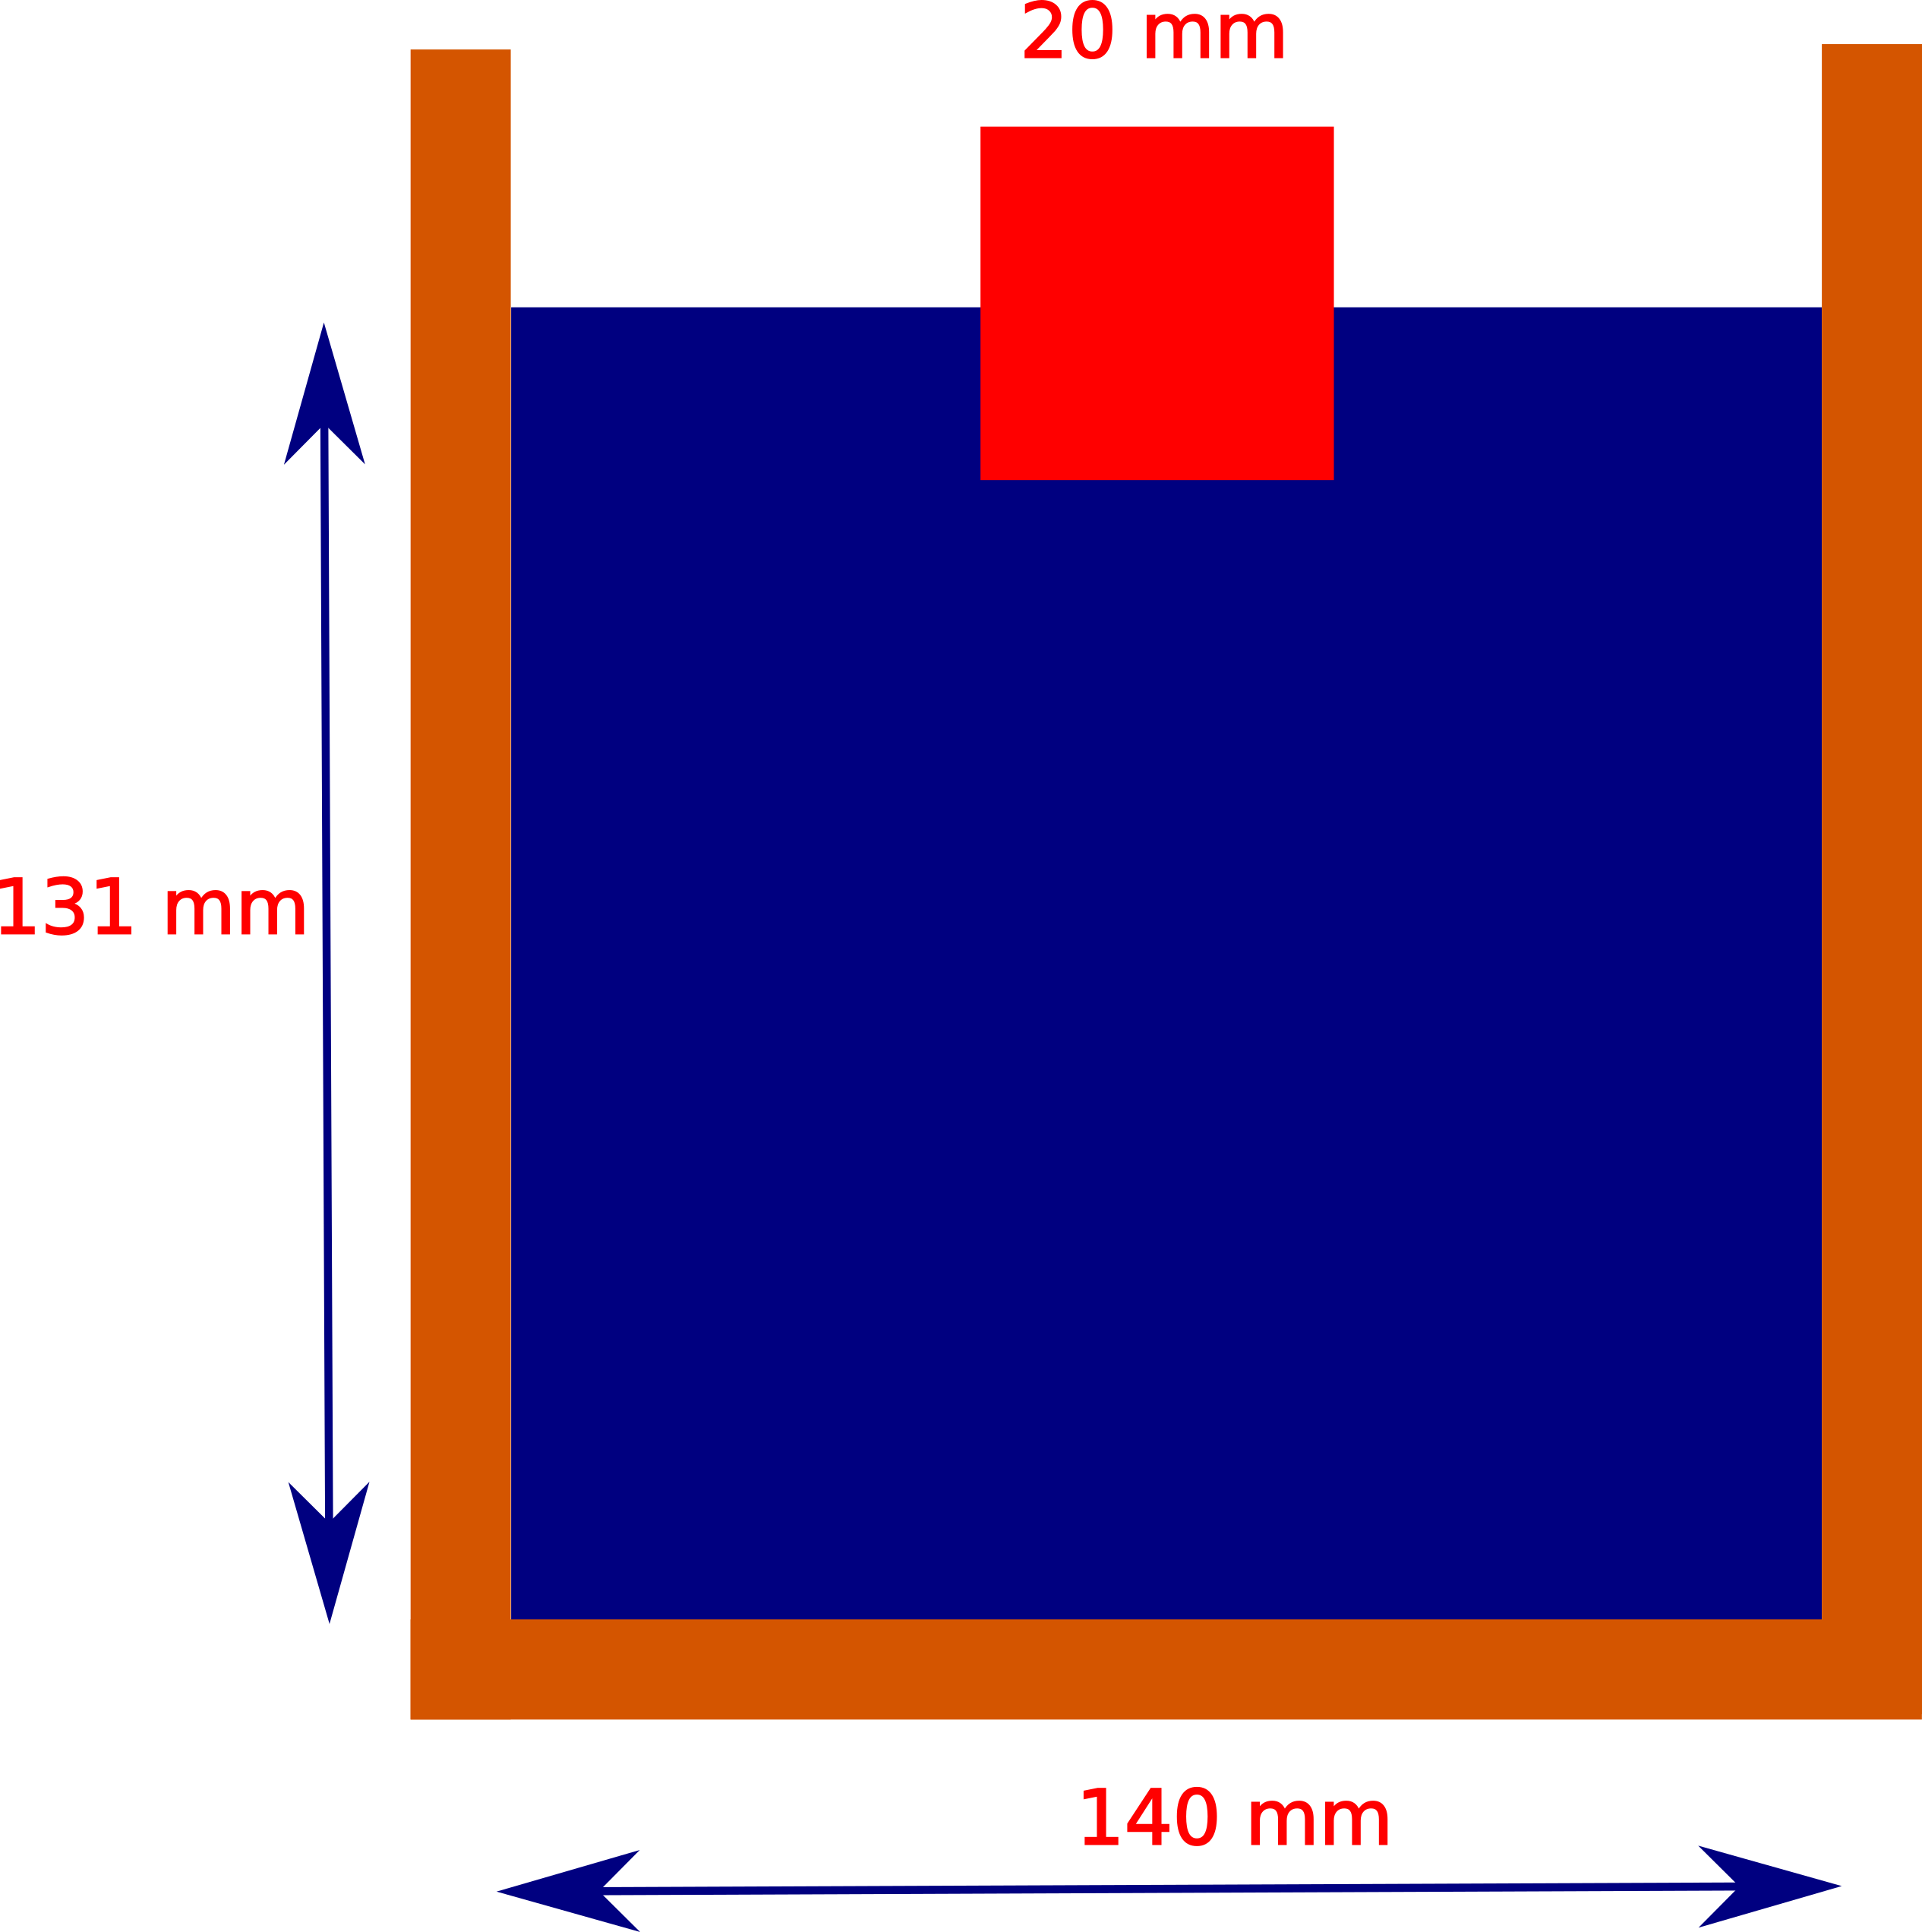
\includegraphics[width=0.4\textwidth]{images/rfc_02_falling_solid_in_water/schematic}
  \caption{Schematic of a cube of density $2120 kg,m\textsuperscript{-3}$
    immersed half way in a steady hydrostatic tank is allowed to settle under
    gravity.}
  \label{fig:results_rfc_02_falling}
\end{figure}



\Cref{fig:results_rfc_02_y_vs_t} shows the evolution of the y-position of
center of mass of the cube, compared against the experimental result by
\citet{wu2014two}. From \cref{fig:results_rfc_02_y_vs_t}, the comparison
reveals a close correspondence between the results obtained by our solver and
the experimental findings, affirming its capability to handle fluid-solid
coupling problems efficiently.
\begin{figure}[!htpb]
  \centering
  \includegraphics[width=0.6\textwidth]{figures/wu_2014_falling_solid_3d/z_vs_t}
  \caption{Vertical position variation of the center of mass of the cube with
    time, compared against the experimental result by \citet{wu2014two}.}
  \label{fig:results_rfc_02_y_vs_t}
\end{figure}

% \FloatBarrier%
% \subsection{RFC validation 3: Falling solid in water}
% \label{sec:rfc_validation_3_falling_solid_in_water}

% zhang2009simulation
% \cite{wu2014two} experimental.
% \cite{qiu20173d} SPH-DEM
% \cite{nan2022cfd} using VOF-DEM


% \FloatBarrier%
% \subsection{RFC validation 3: Force acting on particle in a shear flow}
% \label{sec:rfc_validation_3_single_particle_in_shear_flow}


% \FloatBarrier%
% \subsection{RFC testing 1: Falling circular body in water}
% \label{sec:rfc_testing_1_falling_circular_body_in_water}

% We take a circular body and change the viscosity of the fluid and check the





\FloatBarrier%
\subsection{Mixing of spherical particles in a fluid tank}
\label{sec:mixing-spherical-particles-in-fluid-tank}



\FloatBarrier%
\subsection{Mixing of spherical particles of variable size in a fluid tank}
\label{sec:mixing-spherical-particles-in-fluid-tank}


% \FloatBarrier%
% \subsection{Mixing of spherical particles in a fluid tank with turbine impeller}
% \label{sec:mixing-spherical-particles-in-tank}

% Study of free-surface and solids suspension in top-sealed tanks stirred by
% pitched blade turbine impellers through DEM-VOF method
% This paper has an example of mixing problem.


\FloatBarrier%
\section{Conclusions}
\label{sec:conclusions}


% \section*{References}


\bibliographystyle{model6-num-names}
\bibliography{references}
\end{document}

% ============================
% Table template for reference
% ============================
% \begin{table}[!ht]
%   \centering
%   \begin{tabular}[!ht]{ll}
%     \toprule
%     Quantity & Values\\
%     \midrule
%     $L$, length of the domain & 1 m \\
%     Time of simulation & 2.5 s \\
%     $c_s$ & 10 m/s \\
%     $\rho_0$, reference density & 1 kg/m\textsuperscript{3} \\
%     Reynolds number & 200 \& 1000 \\
%     Resolution, $L/\Delta x_{\max} : L/\Delta x_{\min}$ & $[100:200]$ \& $[150:300]$\\
%     Smoothing length factor, $h/\Delta x$ & 1.0\\
%     \bottomrule
%   \end{tabular}
%   \caption{Parameters used for the Taylor-Green vortex problem.}%
%   \label{tab:tgv-params}
% \end{table}

%%% Local Variables:
%%% mode: latex
%%% TeX-master: "paper"
%%% fill-column: 78
%%% End:
